%!TEX root = these.tex

\chapter[La représentation sémantique comme support de l'intégration de la visualisation et de l'analyse dans un contexte immersif]{La représentation sémantique comme support de l'intégration de la visualisation et de l'analyse en contexte immersif}
\label{Sec:visuAna}
\minitoc
\cleardoublepage

% \bibliography{/Users/trellet/Documents/Manuscript_these/these}
%% Commentaire : la commande \texorpdfstring permet de déclarer un titre de
%% chapitre (ou section, sous-section) alternatif en texte seul, si besoin, qui
%% est utilisé par hyperref pour fabriquer un menu dans les fichiers compilés

%\chapter{\texorpdfstring{Contrôle gestuel de l'articulation}{Contrôle gestuel de l'articulation}}
%% Commentaire : la commande \texorpdfstring permet de déclarer un titre de
%% chapitre (ou section, sous-section) alternatif en texte seul, si besoin, qui
%% est utilisé par hyperref pour fabriquer un menu dans les fichiers compilés

%Exemple de notation qui sera reprise dans l'index : soit $\Q$\index{Q@$\Q$} le corps des nombres rationnels.

% % Intro Visu Analytics
% \subsection{Visualisation analytique}

% L'association étroite entre la visualisation d'informations scientifiques et les analyses associées, dans un même espace et simultanément, met en avant des techniques de visualisation connues et souvent définies en visualisation analytique. Cette discipline récente a en effet pour but de faciliter l'analyse visuelle de données complexes et/ou scientifiques et se définie par le "raisonnement analytique au travers d'interfaces visuelles interactives" \cite{cook_illuminating_2005}. Elle se place à la frontière de nombreux domaines de visualisation, d'interaction ou de perception afin de mettre en avant des informations qui n'auraient pu apparaître lors de l'utilisation cloisonnée des différents domaines mis en jeu. La visualisation analytique s'appuie sur des méthodes de visualisation simples et compréhensibles par l'être humain auxquelles elle ajoute une dimension interactive afin de les relier entre elles. Elle s'inspire donc par plusieurs niveaux aux études d'interactions homme-machine dont la réalité virtuelle s'inspire également \cite{arias-hernandez_visual_2011}. Son principal but est de mettre l'être humain au centre d'une boucle de décision qui sera facilitée par la mise en relation de données de différentes natures et de différentes sources. Ce contexte de travail généré par la visualisation analytique doit être cohérent pour le chercheur. C'est à ce niveau que le domaine de la perception et des études cognitives interviennent afin d'assurer une pleine compréhension et utilisation de l'espace de travail.

% \begin{figure}
%   \centering
%   {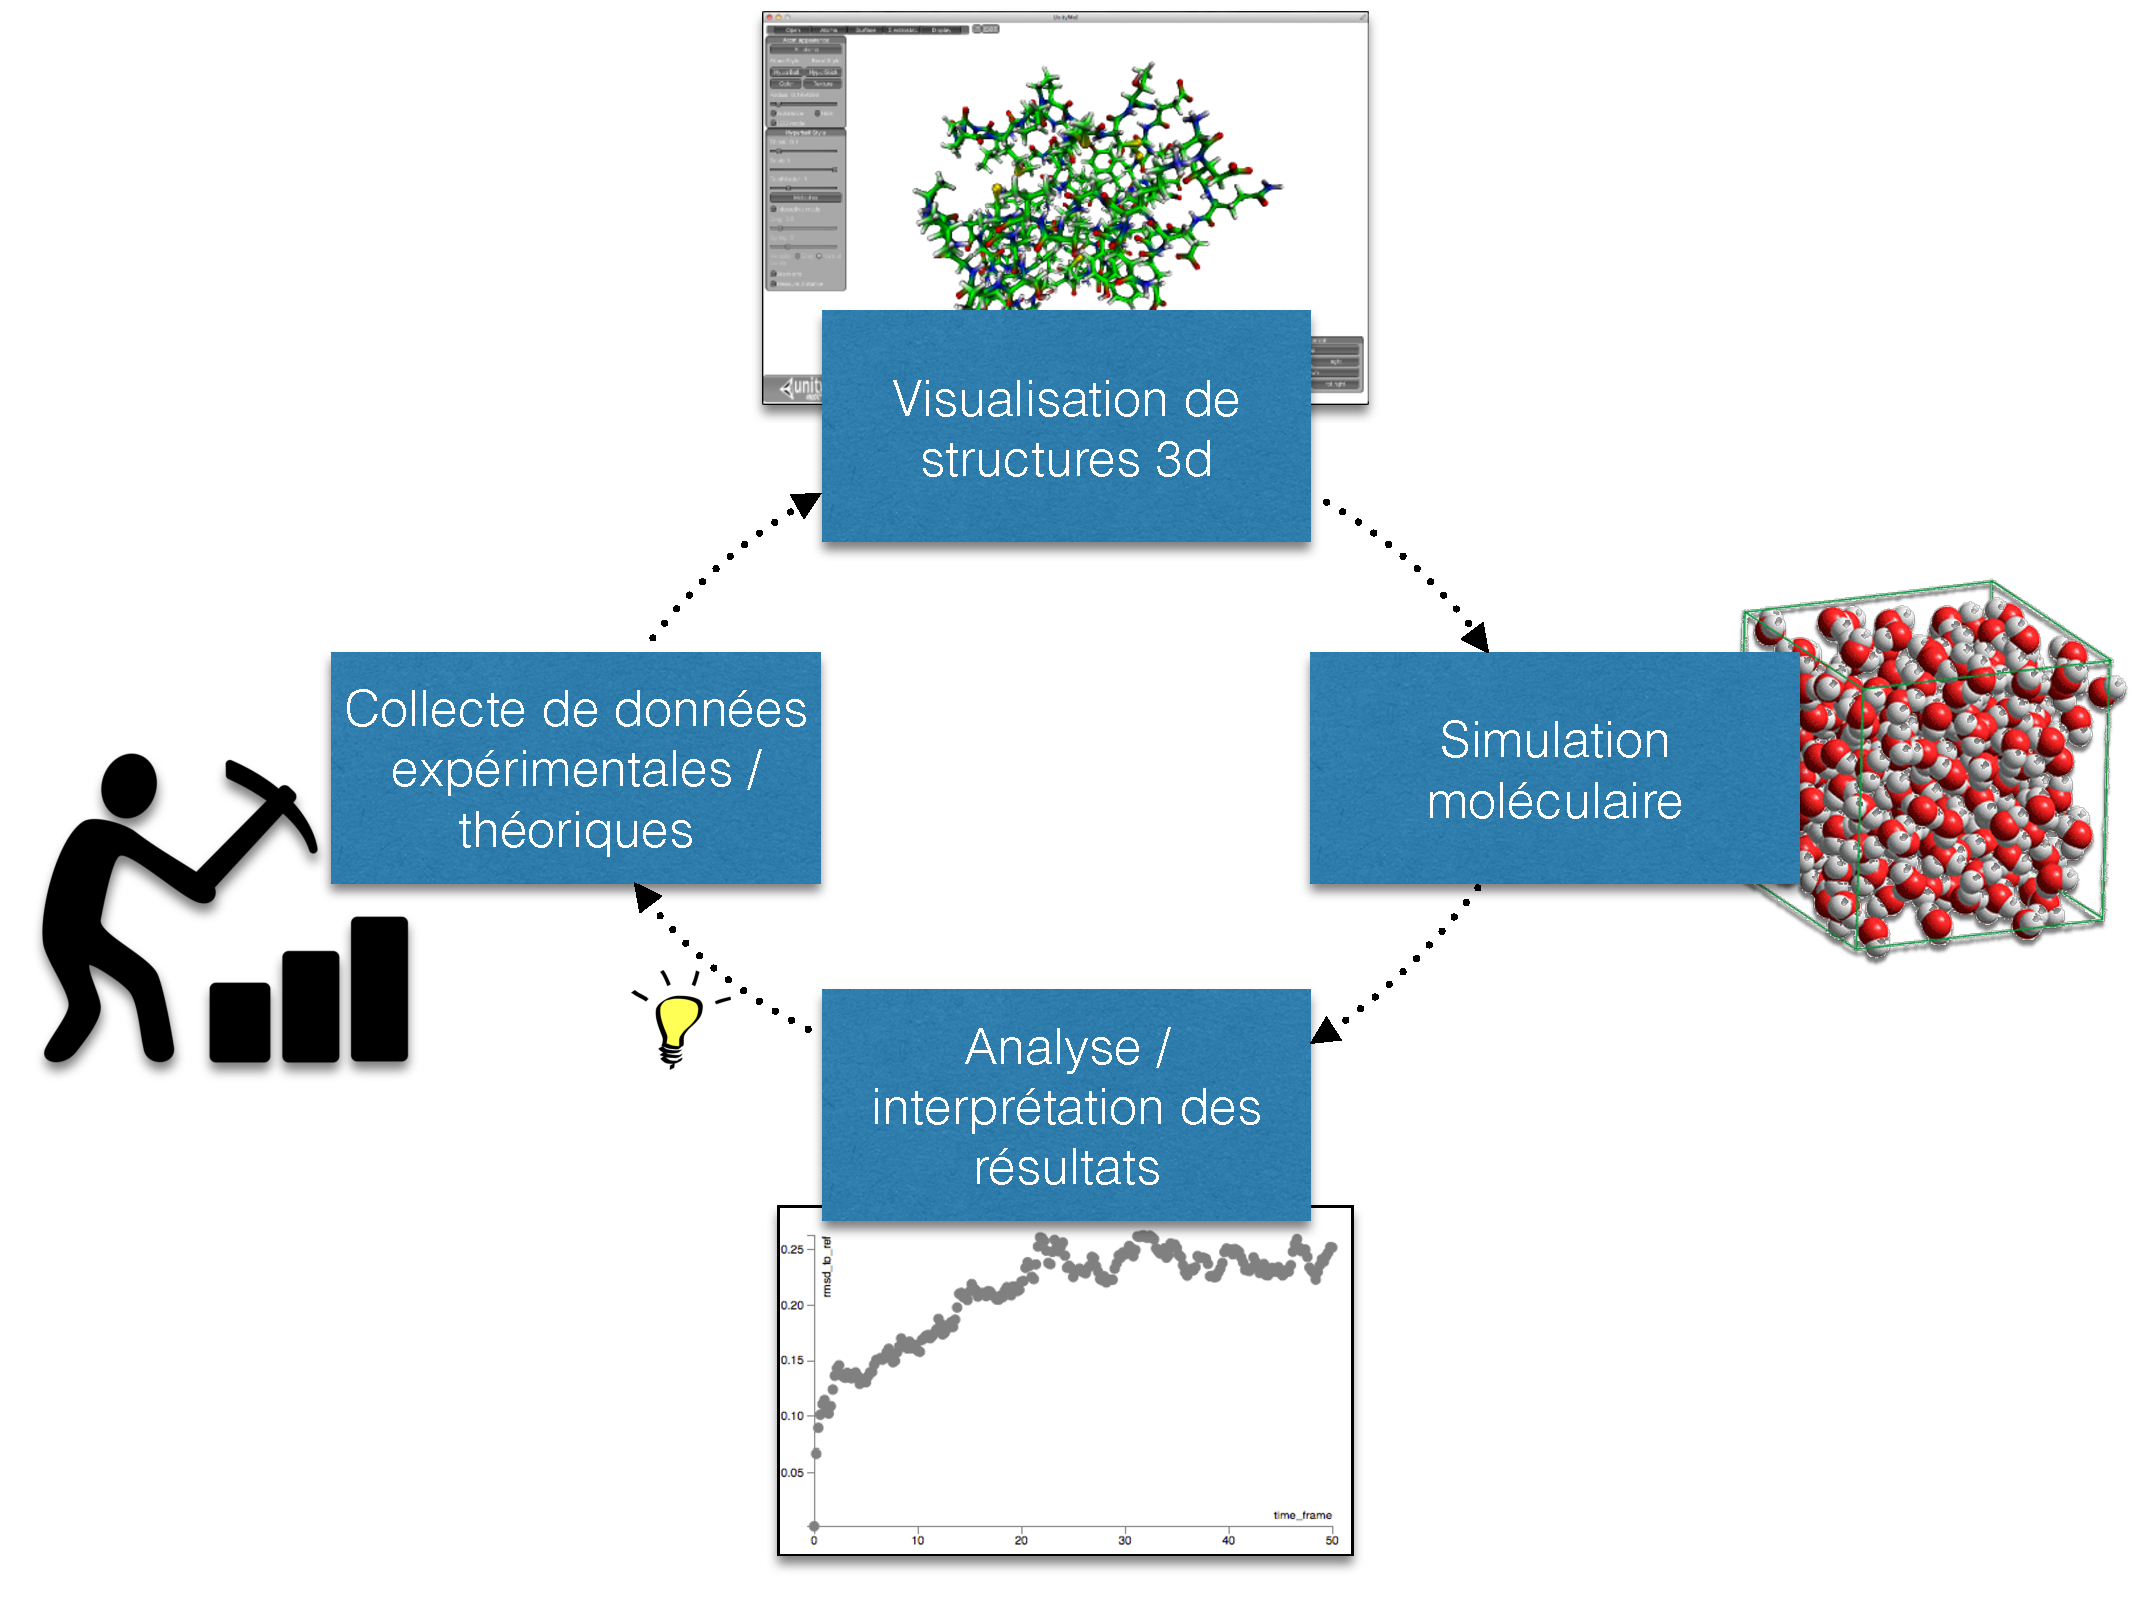
\includegraphics[width=.75\linewidth]{./figures/ch4/ch4_structural_biology_process}}
%     \caption{{\it Processus séquentiel standard de l'étude d'un système moléculaire en biologie structurale.}}
%   \label{Fig:schema_seq_bio_struct}
%   \hspace{0.3cm}
% \end{figure}

% \begin{figure}
%   \centering
%   {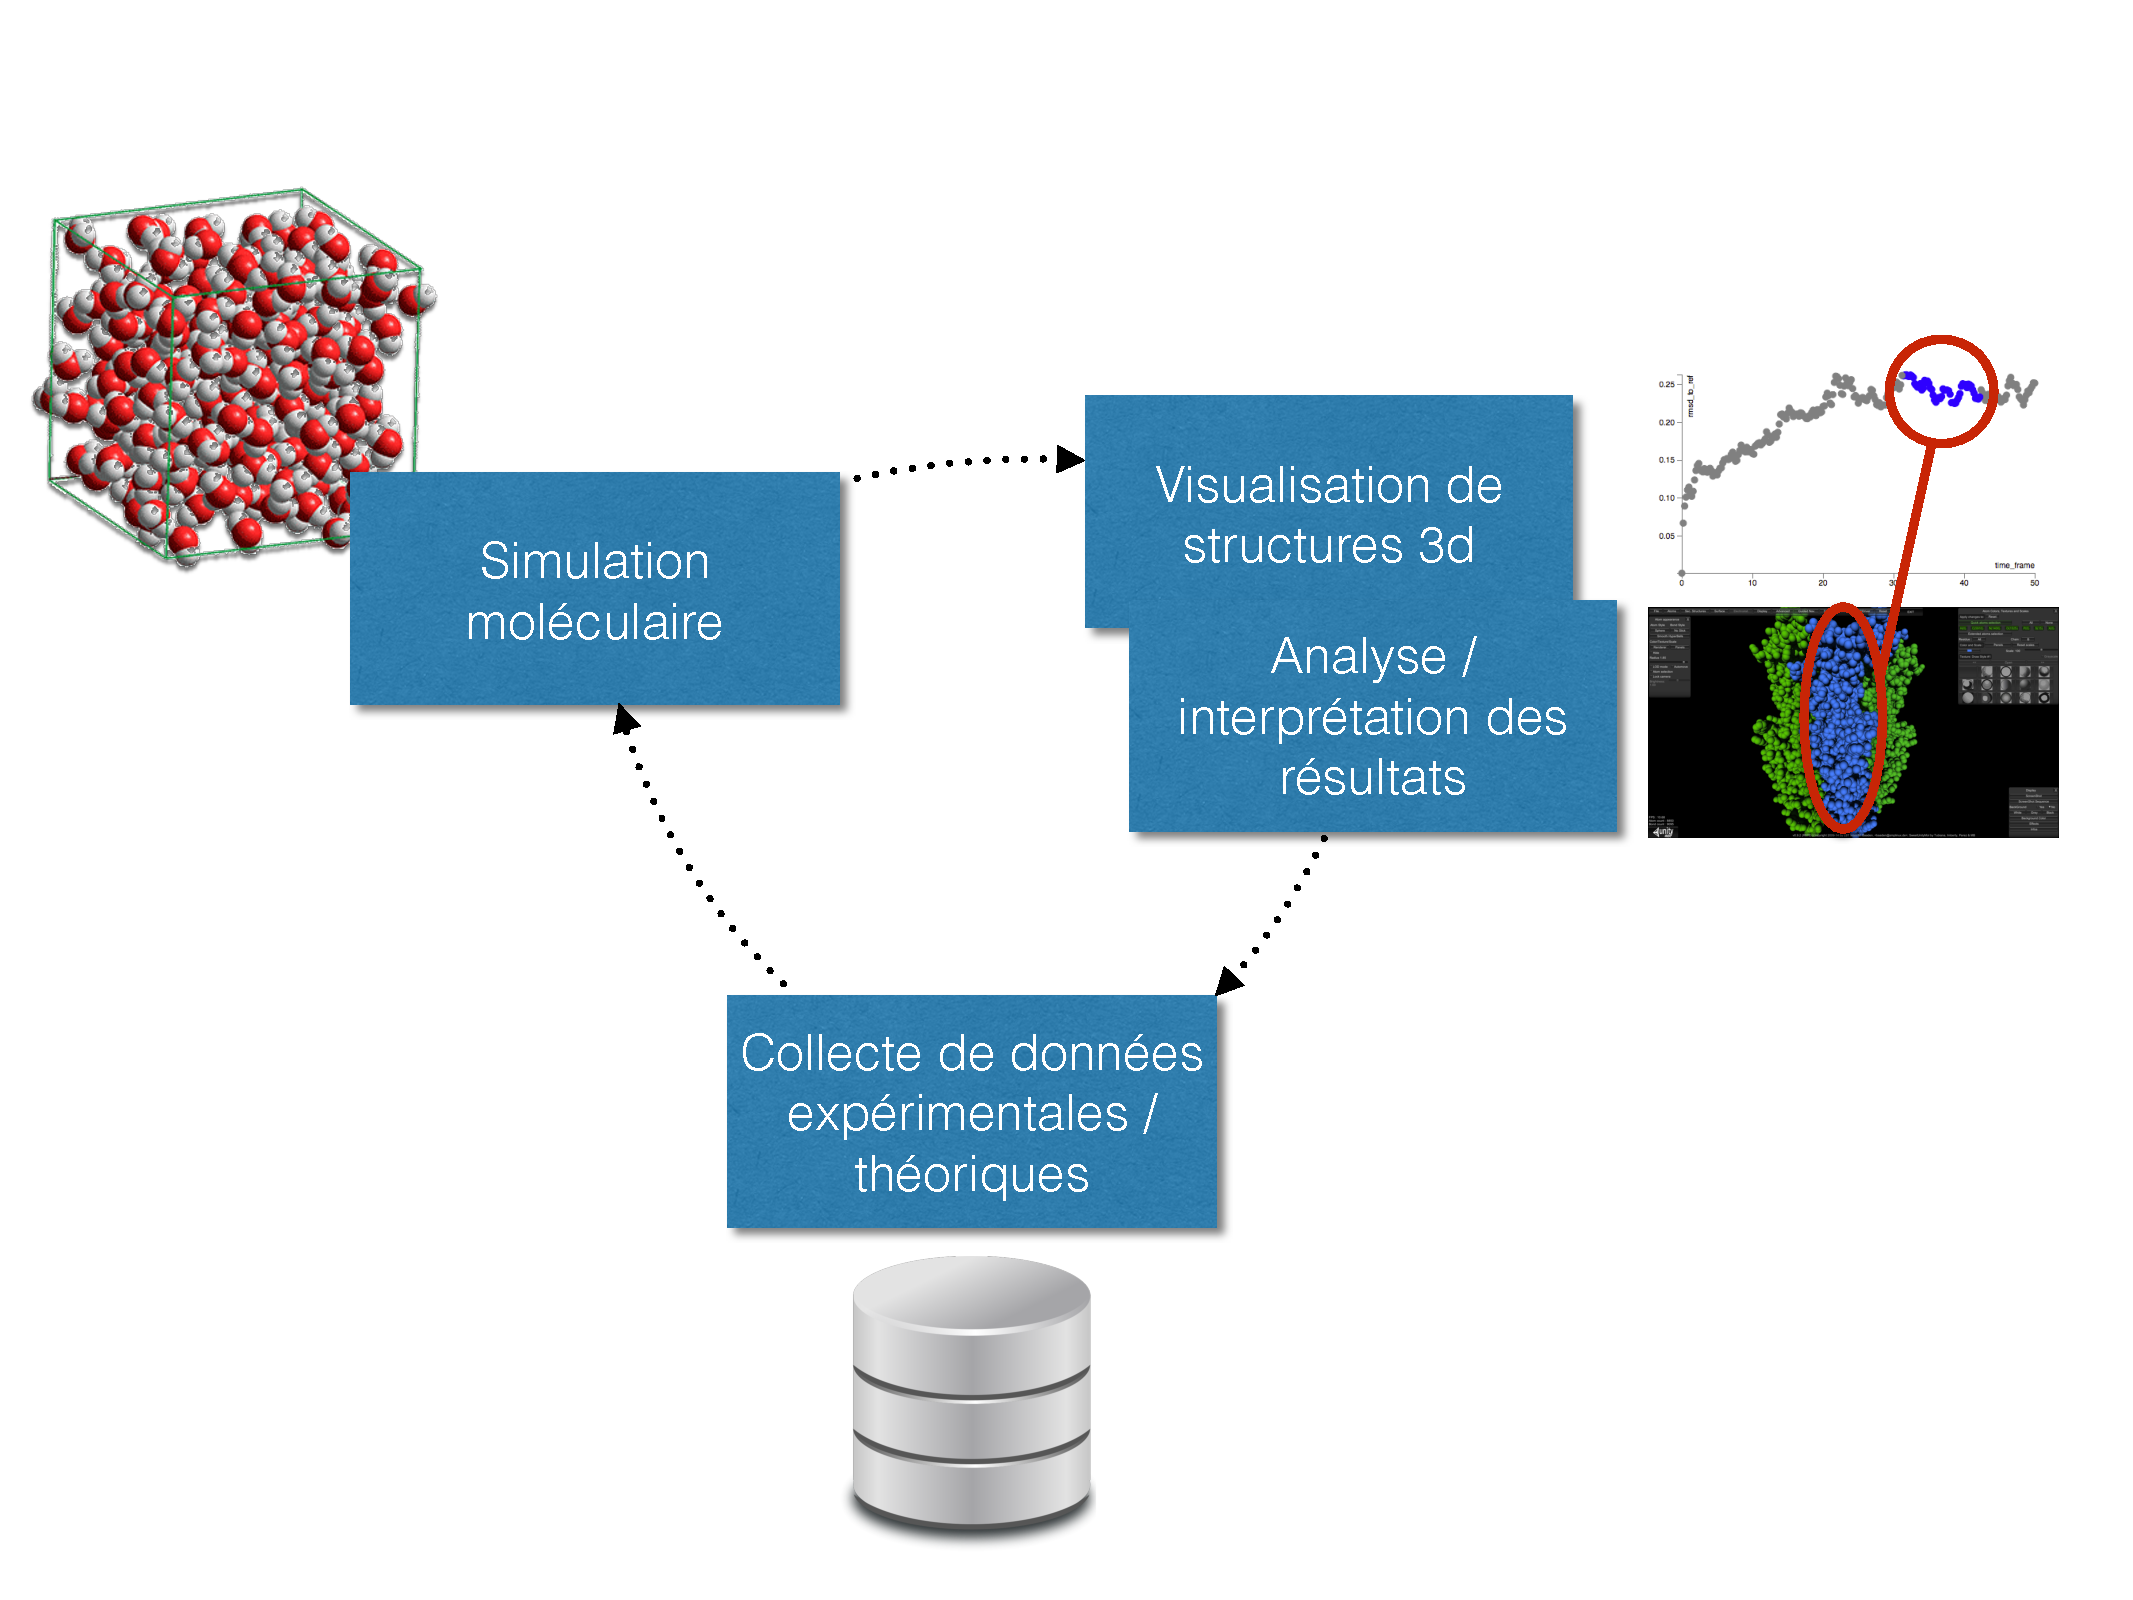
\includegraphics[width=.75\linewidth]{./figures/ch4/ch4_structural_biology_optim.pdf}}
%     \caption{{\it Processus séquentiel optimisé pour l'étude d'un système moléculaire en biologie structurale.}}
%   \label{Fig:schema_seq_bio_optim}
%   \hspace{0.3cm}
% \end{figure}

% La visualisation analytique vise donc à combiner la visualisation de données passées en entrée et leurs analyses afin de créer de nouvelles connaissances qui pourront elles-mêmes être utilisées par la suite en entrée de la boucle. Ce processus, expliqué par Keim et al. \cite{keim2010mastering}, forme ainsi une boucle d'analyse fermée qui vient raccourcir considérablement la boucle habituelle présentée dans la figure X. Une nouvelle représentation de cette boucle intégrant la visualisation analytique peut être observée dans la figure Y.

% % Intro sémantique / données liées
% \subsection{Représentation des connaissances}

\section{Liste des figures}

\begin{enumerate}
	\item Boucle séquentielle de la biologie structurale
	\item Boucle avec visualisation analytique
	\item Overview+Detail dans Google Maps (?)
	\item Focus+Context via sélection dans plot reflétée dans d'autres plots
	\item Sélection dans visu 3d entraîne points concernés highlighté dans visu 2d
	\item Ontologie OWL
	\item Triplets RDF présent dans base de donnée
	\item 5 requêtes SPARQL pour classification des mots-clés du moteur de traduction
	\item Schéma de l'application
	\item Structure 3d GLIC+bromoforme
	\item Requêtes SPARQL analyses simples/complexes - TO DO
	\item Temps d'exécution des différentes actions au sein de l'application - TO DO
\end{enumerate}

%\section{Introduction}

Nous avons vu dans le chapitre 1 que dans le schéma standard de l'étude d'un phénomène biologique à l'échelle atomique, la mise en place d'hypothèses de travail se fait suite à l'analyse standardisée d'une simulation moléculaire. Cette simulation, dans le meilleur des cas, aura mis en avant plusieurs pistes de réflexion provenant de changements structuraux ou énergétiques du complexe moléculaire d'intérêt. Cependant, la majorité des simulations amènent que peu d'informations utilisables pour émettre de nouvelles hypothèse et seule une suite de simulations dont les paramètres ont évolué progressivement permet de dégager un résultat significatif. La simulation et son analyse sont donc deux des quatre tâches identifiées dans la boucle séquentielle de la biologie structurale que nous avons exposé en introduction. La succession de simulation->analyse->nouveaux paramètres->simulation->analyse... est un processus long et coûteux. Tant en terme de quantité de données à traiter qu'en terme de temps de traitement et de communication des données. Notre approche vise à raccourcir ce processus en combinant simulation et analyses afin de:
\begin{enumerate}
    \item Identifier et reconnaître les acteurs biologiques importants d'une simulation de façon rapide mais complète
    \item Réduire la quantité de données générée afin de ne garder que la partie pertinente pour les hypothèses
    \item Apporter à l'utilisateur les outils de décision adaptés en lui fournissant les liens logiques entre ses données
    \item Orienter la simulation vers des paramètres plus pertinents suivant les décisions de l'utilisateur
\end{enumerate}

Notre but est donc de placer l'utilisateur au centre d'une boucle de décision dont les deux principaux fournisseurs de données seraient les changements structuraux induits par la simulation et les analyses physico-chimiques et statistiques associées. Ces deux moteurs seraient directement dirigés et manipulés par l'utilisateur suivant les hypothèses et les conclusions qu'il tirerait des données résultantes de leur combinaison.

Ce raccourcissement du processus d'étude d'une protéine est aussi motivé par l'espace de travail que l'on lui dédie. En effet, la réalité virtuelle doit par nature se défaire du carcan clavier/souris et mettre en jeu des techniques d'interaction directes plus naturelles. Le nombre brut de commandes possibles pour interagir avec l'environnement est réduit comparé aux possibilités qu'offrent des conditions de bureau standards. L'ensemble des actions impliquant l'utilisation d'une souris ou d'un clavier (ou une combinaison des deux) ne peut être géré dans sa totalité par un mécanisme d'interaction associé à un périphérique adapté à l'immersion, à des commandes gestuelles ou vocales. La combinaison de la richesse des données à analyser et du nombre important de contrôles propre à la visualisation moléculaire où les possibilités de rendus et de manipulation des objets sont très nombreuses empêchent la mise en place en RV d'une structure logicielle copiant la structure des solutions standards pouvant exister. Il est donc nécessaire, en parallèle de la mutualisation des activités de visualisation et d'analyse, de mutualiser également les actions de contrôle afin de réduire le nombre d'étapes d'interaction que l'utilisateur devra effectuer pour arriver à un résultat. En plus de l'apport en simplicité, cette mutualisation permet de s'affranchir d'un maximum de dispositifs d'interaction qui viendraient réduire l'immersion pour l'utilisateur. De nombreuses recherches en interaction homme-machine ont tenté de répondre à cette problématique et plusieurs solutions matérielles et logicielles existent afin de prendre en compte des signaux naturels (mouvements ou voix par exemple) en entrée afin de permettre la mise en place d'actions, même complexes.

Lorsqu'on se concentre sur un domaine d'étude en particulier, cette mutualisation est d'autant plus facile que certaines actions sont communes et peuvent donc être définies dans leur totalité à partir d'un minimum d'éléments en entrée. En effet, la connaissance d'un domaine doit permettre de prédire et de fournir des outils dont l'utilisateur aura besoin suivant l'étape du processus dans laquelle il se trouve et ses actions au sein de celle-ci. Comme nous venons de l'énoncer, cela ne peut se faire qu'à travers une excellent connaissance du métier et du domaine. Notre étude nous a donc mené à nous interroger sur la possibilité de formaliser les concepts qui sont utilisés dans le processus d'étude d'une molécule afin de permettre leur utilisation.

Parmi les différentes techniques de visualisation analytique citées dans la section \ref{visu_ana_tools}, celle du Focus+Context, et plus spécifiquement de la technique du \textit{brush-and-link}, est un candidat pertinent pour mettre en avant des informations supplémentaires obtenues à partir des analyses indépendantes effectuées sur une simulation. En biologie structurale, les résultats d'analyse peuvent souvent être représentés au travers de nuages de points, d'histogrammes ou de diagrammes à bandes. Ces représentations s'adaptent particulièrement bien à la technique du \textit{brush-and-link} puisque la sélection de sous-ensembles y est aisée. De plus, la perspective d'une fenêtre dynamique regroupant le contexte global et les détails dans un même ensemble est particulièrement adapté à un environnement immersif. En effet, l'immersion peut être considérablement impactée, et ce de façon négative, lors du partage spatial du dispositif immersif en plusieurs contextes de travail.
Du point de vue de la visualisation, le but est d'être capable de sélectionner un sous-ensemble structural d'un complexe moléculaire afin de mettre en avant les informations correspondant à ce sous-ensemble dans l'espace d'analyses. Par exemple, et comme illustré dans la Figure \ref{Fig:bilateral_selection}, la sélection d'un ou plusieurs modèles de la trajectoire aura pour conséquence de mettre en avant cette sélection au sein de la structure et de mettre en avant le sous-ensemble, si existant, dans les graphiques d'analyse. Chaque point des graphiques est relié à un niveau hiérarchique structural précis (modèle/chaîne/résidu/atome) et une action sur un ensemble de points aura pour effet d’entraîner une action sur le niveau structural correspondant. 
% Cela ne peut se faire que si des liens existent entre les données structurales 3D et les données analytiques. Il doit exister une correspondance étroite et bilatérales entre les éléments présentés dans le rendu visuel de la structure 3D (atomes, résidus, chaînes, protéines,...) et dans le rendu visuel des analyses (points, barres, surfaces,...) afin de permettre une synchronisation des actions entre les deux espaces de rendus.
Ces outils ne sont pas suffisant à eux seuls pour répondre à notre problématique. En effet, l'idée principale de notre approche vise à mettre en place une plateforme logicielle souple et générique afin de prendre en compte un nombre important de données hétérogènes en entrée sans nécessité de nouveaux développements pour assurer son fonctionnement. Cette généricité doit passer par une certaine automatisation des étapes de liaison entre les données hétéroclites que peuvent être des données dédiées à la visualisation 3D et des données provenant d'analyses ou de propriétés physico-chimiques.

\begin{figure}
  \centering
  {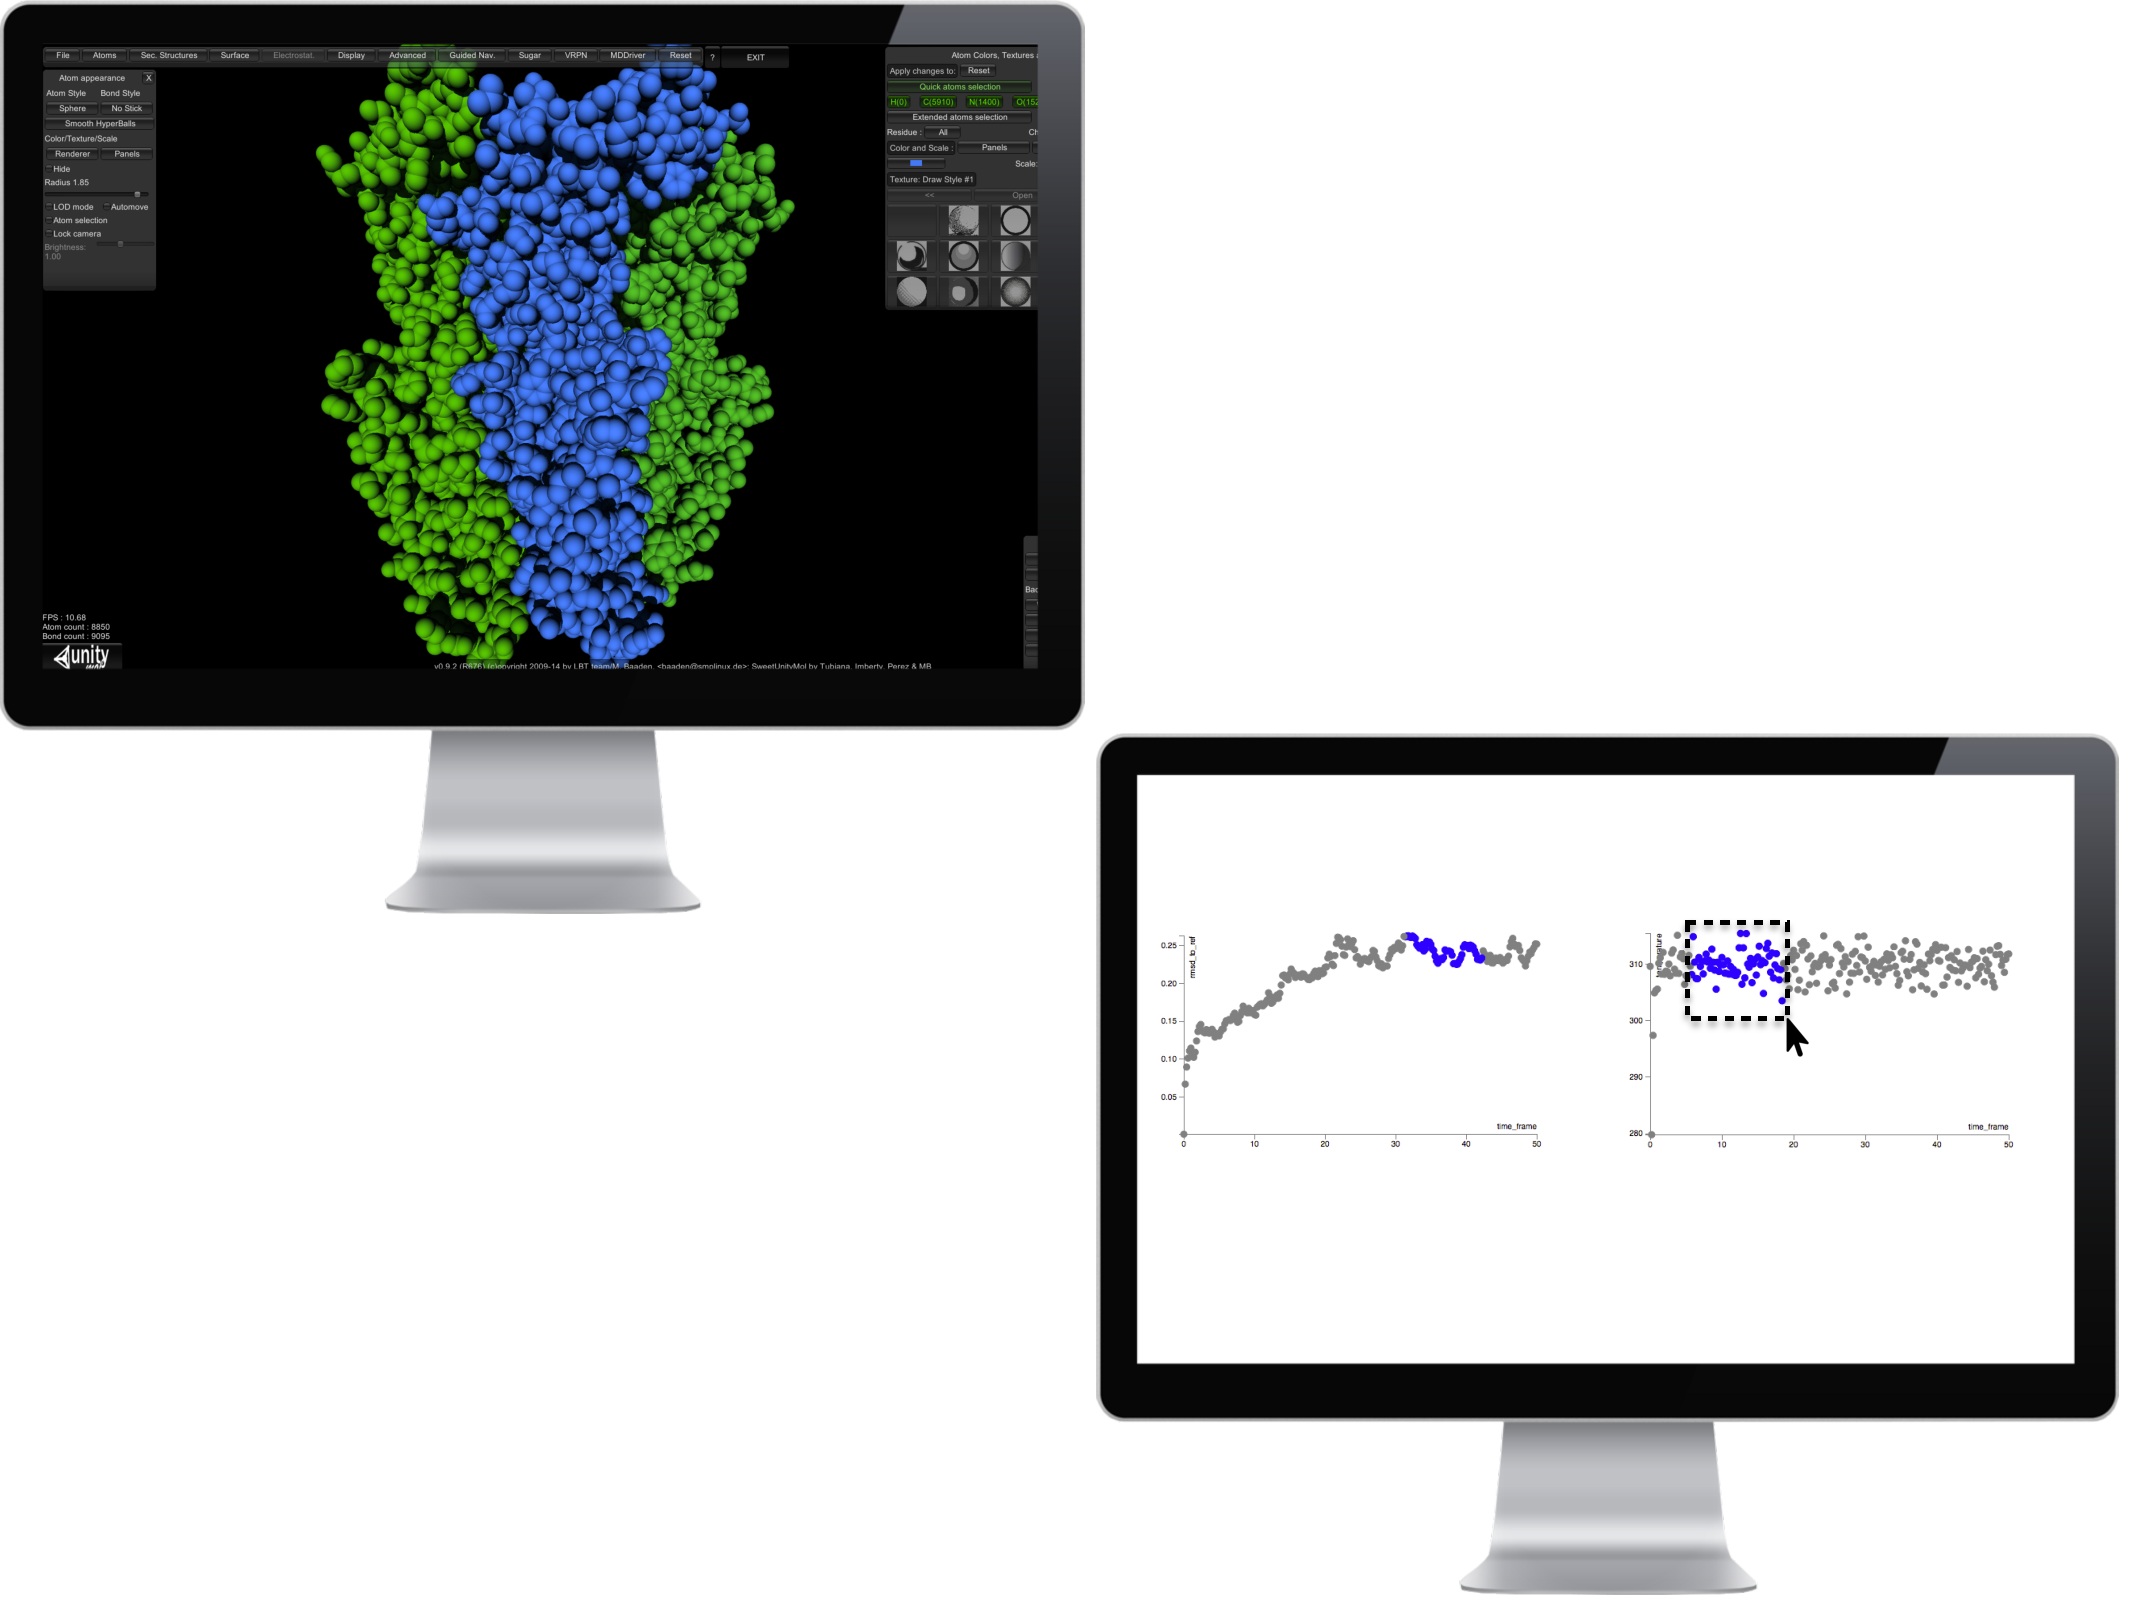
\includegraphics[width=.75\linewidth]{./figures/ch4/ch4_visu2d_visu3d_link}}
    \caption{\it Illustration du lien entre des diagrammes de dispersion présentant deux résultats d'analyses et un visualiseur 3d. Une sélection d'individus dans les diagrammes entraîne une coloration et une mise en avant de la représentation 3d de ces mêmes individus.}
  \label{Fig:bilateral_selection}
  \hspace{0.3cm}
\end{figure}

\section{Sémantique et données liées}

Parmi les solutions possibles, une première pourrait être de mettre en place un suivi strict des données en assignant des identifiants uniques aux données représentant les mêmes concepts afin de garder une cohérence complète entre chaque élément affiché dans l'espace de visualisation et chaque élément de l'espace d'analyse. L'un des problèmes de cette solution se trouve dans la possibilité pour les espaces d'évoluer rapidement et demande donc ainsi une évolution constante du pool d'identifiants. De plus, aucune information quant à la structure du complexe moléculaire ne serait extractible de ces identifiants, une gestion spécifique cherchant à maintenir la cohérence entre les identifiants du premier espace et les identifiants du second devrait ainsi être mise en place en parallèle.
Une seconde solution est de donner au programme un couche d'abstraction supplémentaire via une définition ontologique des concepts manipulés afin de lui permettre de savoir quel concept est concerné par une éventuelle action (sélection, mise en avant, mise en arrière-plan, ...). Chaque élément avec lequel interagit l'utilisateur correspond à un individu unique dont la nature ou l'une de ses propriétés est mise en avant, soit à travers une représentation visuelle, soit à travers une représentation analytique. Chaque interaction avec cet individu déclenchera un résultat dans tous les espaces affichant au moins une de ses propriétés.
Il est donc nécessaire de mettre en place un vocabulaire générique que manipulera la plateforme et que l'utilisateur aura simplement à remplir avec ses données spécifiques afin de former une base de données permanente décrivant son système. 
Les concepts mis en jeu au sein de la plateforme doivent être correctement définis pour que l'utilisateur sache comment enrichir la base de données qui sera prise en entrée par les modules et afin que les données puissent être liées entre elles de façon optimale. La mise en place d'une ontologie permet que ces deux prérequis soient respectés. Le web sémantique tend à lier et structurer les données de façon à faciliter l'accès aux connaissances qu'elles contiennent. C'est également le but de notre étude et il semble donc adapté de reprendre les principes de cette approche afin de mettre en place la structure de notre base de données. Plusieurs avantages qu'offre la mise en place de données liées et d'une ontologie définissant les concepts étudiées peuvent être énumérés:

\begin{itemize}
    \item La plateforme peut identifier à chaque étape les concepts mis en jeu par l'utilisateur et donc proposer des actions adaptées
    \item L'utilisateur dispose d'une définition précise de l'implémentation des concepts et peut ainsi fournir ses données en accord avec celle-ci
    \item Il est possible de partager les données utilisées puisqu'elles sont clairement définies par une ontologie
    \item Les liaisons entre les concepts définies dans l'ontologie peuvent être utilisés à l'identique pour relier des modules différents (visualisation/analyses/interactions/...)
    \item La base de données primaire créées à partir des données de l'utilisateur peut évoluer à chaque instant et grandir grâce à de nouvelles données obtenues à partir des premières
\end{itemize}

Nous avons choisi comme support de représentation des données manipulées au sein de notre plateforme, la structure provenant du Web Sémantique basé sur le modèle RDF. L'avantage du langage RDF est sa possibilité d'être étendu et structuré grâce à une couche ontologique appelée \textit{Web Ontology Laguage} (OWL) qui reprend les critères standards des ontologies existantes et qui est le support de nombreuses ontologies recensées dans le portails officiels de bio-ontologies largement utilisées dans la communauté scientifique \cite{smith_obo_2007}. Le modèle RDF a également l'avantage de se baser sur une approche de logique de description permettant d'étendre les connaissances d'une base de données via des relations logiques définies dans l'ontologie sans que ces relations factuelles soient explicitement présentes dans la base de données.

\begin{figure}
  \centering
  {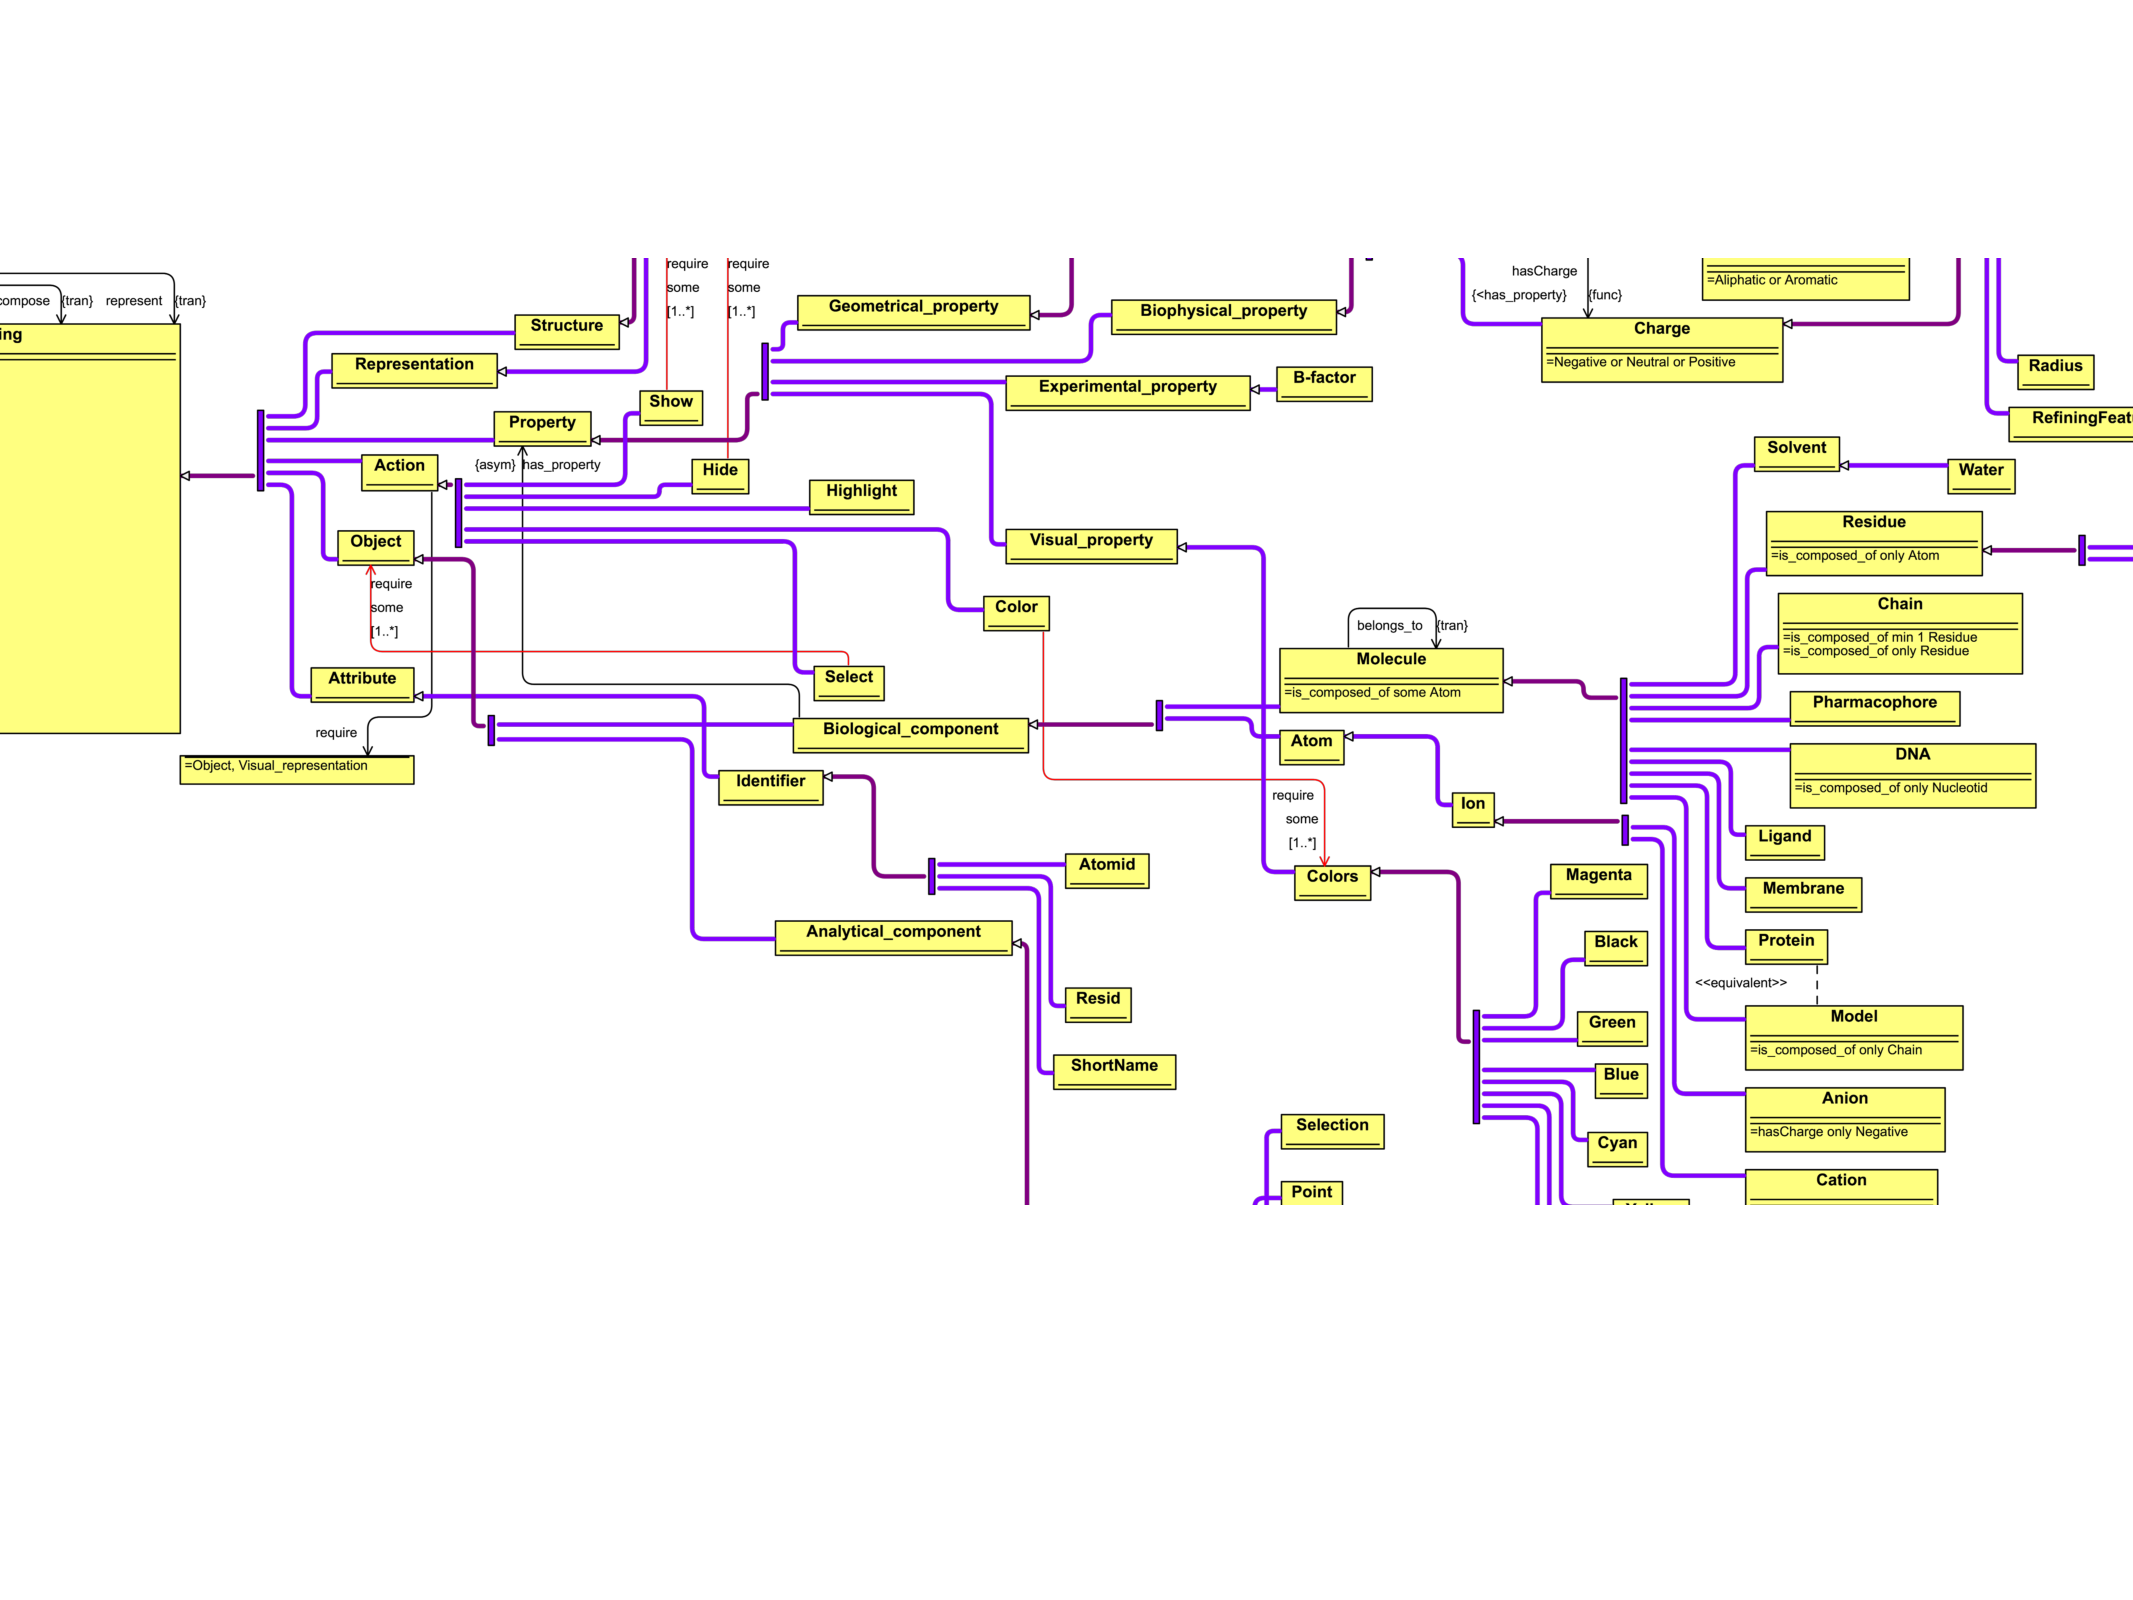
\includegraphics[width=.75\linewidth]{./figures/ch4/ch4_ontology.pdf}}
    \caption{\it Extrait de l'ontologie OWL créée pour la mise en place de notre représentation sémantique de la plateforme logicielle. Visualisation obtenue avec OWLGrEd \cite{barzdins2010owlgred}}
  \label{Fig:extract_OWL_ontology}
  \hspace{0.3cm}
\end{figure}

\subsection{Ontologie OWL}

Comme le montre la Figure \ref{Fig:ontology}, nous avons essayé de définir de façon complète l'ensemble des concepts que l'utilisateur aurait à manipuler lors de ses activités de visualisation et d'analyses synchronisées. 
Nous l'avons vu auparavant, plusieurs bio-ontologies ont été mises en place ces dernières années. Afin d'avoir une description la plus précise qui soit des concepts biologiques mis en jeu, nous nous sommes appuyés sur une ontologie déjà existante et disponible en ligne décrivant de façon complète les acides aminés et leurs propriétés \footnote{\url{http://bioportal.bioontology.org/ontologies/AMINO-ACID}}. Cette ontologie nous a permis de poser les bases biologiques d'un des principaux concepts de biologie structurale. En rassemblant des informations telles que la taille, l'hydrophobicité ou bien la charge de chaque acide-aminé il est ainsi possible d'extraire rapidement des groupes d'acides aminés possédant les mêmes propriétés et ainsi utiliser ces propriétés pour des raisonnements complexes lors de l'interrogation de la base de données. Parmi les nombreuses autres bio-ontologies disponibles, aucune d'entre-elles parvenait à définir aussi simplement que nous le désirions les autres concepts dont nous avions besoin. Leur complexité souvent beaucoup trop importante aurait rapidement surchargé notre ontologie. Nous avons donc créer notre propre définition de ces concepts et ainsi éviter un surplus considérable de concepts/propriétés inutilisés provenant d'ontologies trop précises. Il est cependant important de noter qu'une extension de notre ontologie est possible et même encouragée. Cette extension pourrait par exemple compléter et étoffer certaines propriétés biologiques intéressantes pour des études précises.
En plus des concepts biologiques cités précédemment, nous avons également cherché à définir tous les concepts d'analyses et d'action qui seront en jeu lors de la session d'utilisation de notre plateforme. Les actions rassemblent toutes les actions que l'utilisateur pourrait vouloir effectuer avec les données qu'il manipule, de façon directe ou indirecte. Elles reprennent essentiellement les commandes permises par les logiciels de visualisation moléculaire et les outils d'analyse que nous utilisons. Dans les concepts analytiques sont rassemblés les éléments graphiques ou abstraits qui rentrent en jeu dans la création et la visualisation d'un résultat d'analyse. Nous ne définissons pas, volontairement, les processus d'analyse eux-mêmes car ceux-ci peuvent être de natures très différentes et possèdent un champ de définition bien trop large et complexe pour le sujet de cette thèse. De plus, nous séparons volontairement la visualisation des résultats d'analyses des processus/modules d'analyses. Cela ne signifie pas que certains processus d'analyses ne seront pas utiliser au sein de la plateforme logicielle, il n'est simplement pas pertinent de les ajouter à l'ontologie dans le but d'uniformiser les rendus 3D et d'analyses.

\begin{figure}
  \centering
  {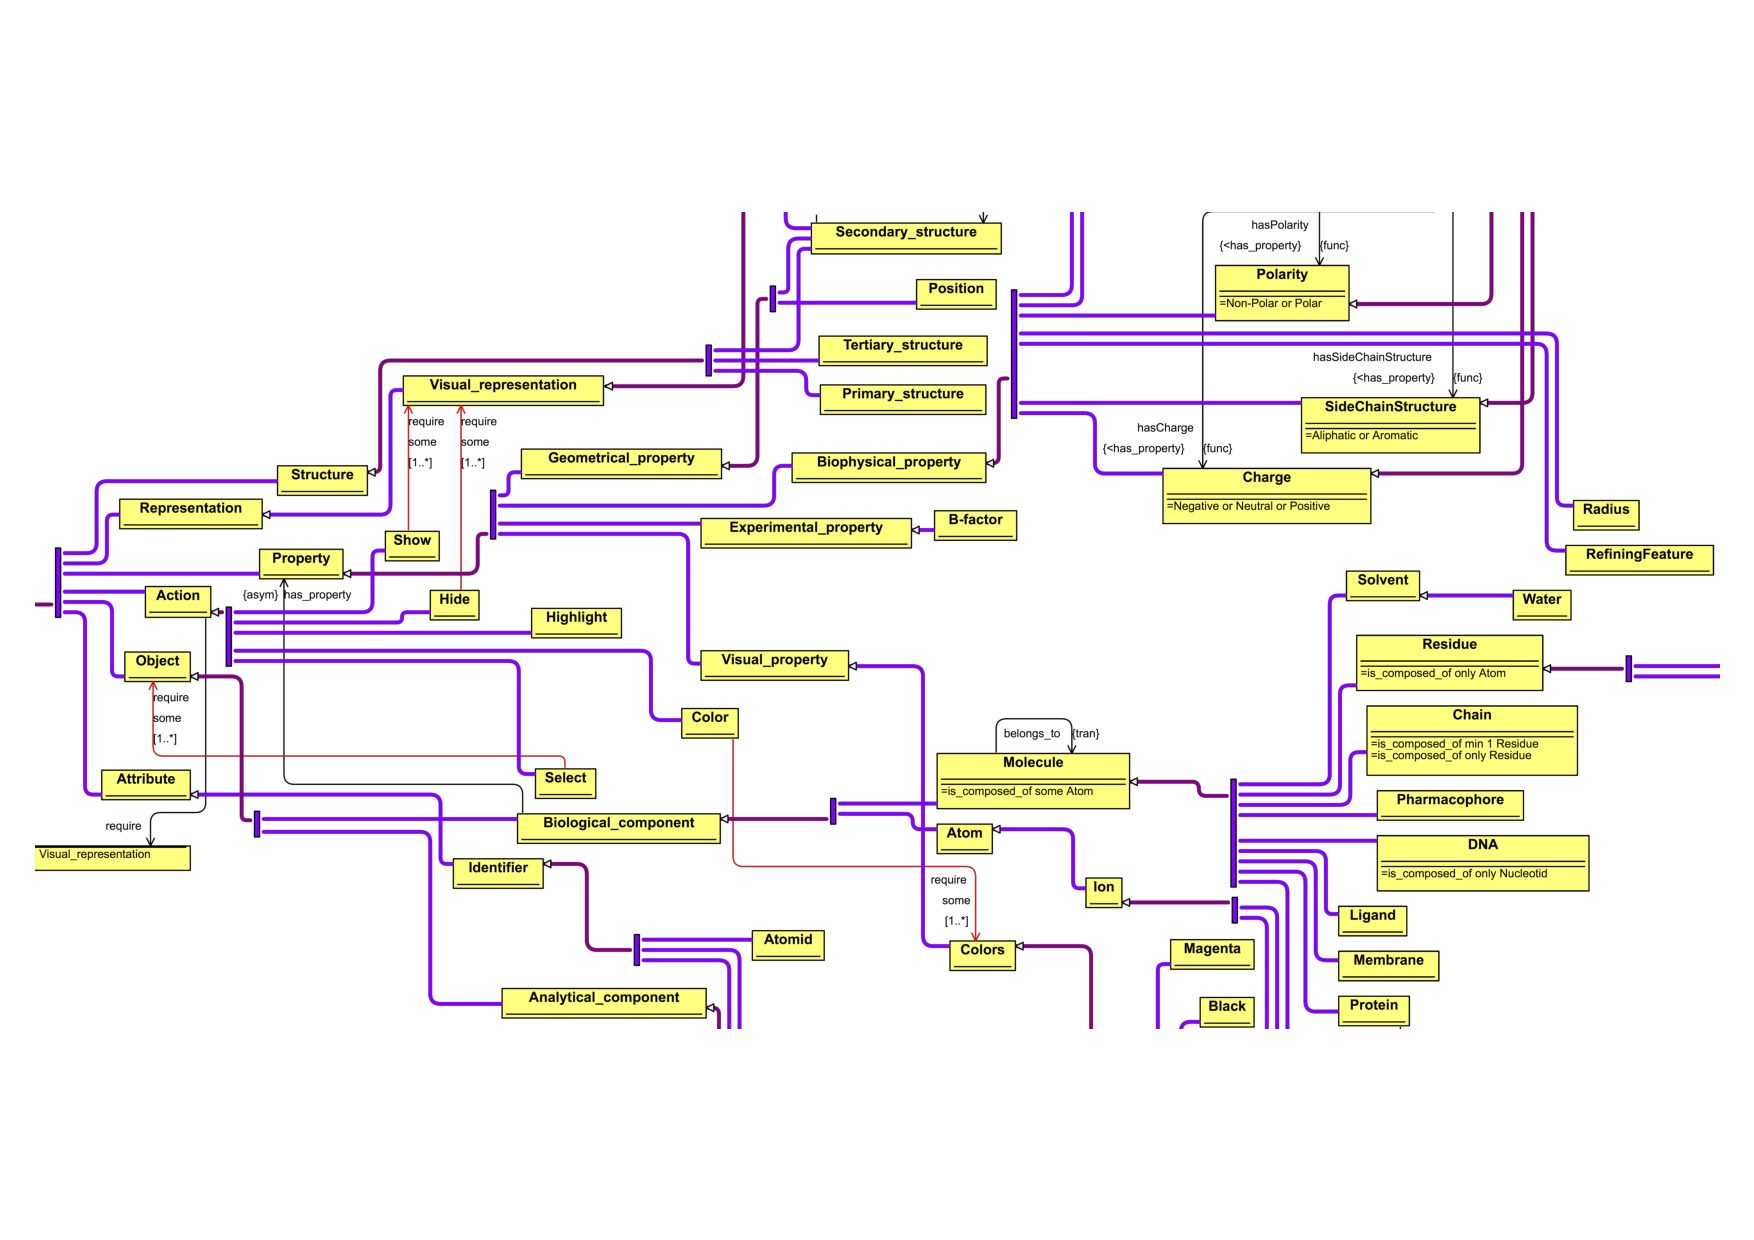
\includegraphics[width=.75\linewidth]{./figures/ch4/ontology}}
    \caption{\it Sous-partie de la représentation sous forme de graphe de l'ontologie créée dans le cadre de notre étude. Les cadres jaunes désignent les classes dont les liens de type (est-un) sont représentés par des flèches orientées. La complexité d'une telle représentation est telle qu'il est très difficile de regrouper dans un même espace l'ensemble des classes et des propriétés définies dans une ontologie complète.}
  \label{Fig:ontology}
  \hspace{0.3cm}
\end{figure}


Une fois l'ontologie mise en place, il est possible d'alimenter la base de connaissance en ajoutant les informations biologiques regroupées par l'expert scientifique. Ces informations vont devoir respecter le vocabulaire et la classification définie par les règles présentes dans l'ontologie OWL.

\subsection{Base de données RDF/(S)}

La description d'un environnement d'intérêt passe par l'analyse de toutes les informations biologiques pouvant être labellisées par une chaîne de caractère ou une valeur et qui correspond à un concept ou une propriété identifiée dans l'ontologie OWL. Chaque information alimentera une base de données RDF organisant toutes les informations, de la même manière que pour les descriptions ontologiques, sous forme de triplets de type Sujet/Propriété/Objet.
Dans le cas qui nous intéresse pour ce travail de thèse, les simulations numériques moléculaires peuvent être découpées en une succession de modèles statiques 3D successifs. Chaque modèle correspond à l'échelle \textit{Model} décrite dans notre ontologie. C'est le groupe structurel le plus large que nous ayons défini dans les composants structurels biologiques. Plusieurs triplets présents dans notre base de données finale sont illustrés dans le Listing \ref{rdf_xml}. Chaque atome possède une position 3d ainsi qu'un résidu auquel il appartient et indirectement, de la même manière, une chaîne et un modèle de référence grâce aux règles d'inférence. Cette information n'a donc pas besoin d'être spécifiée puisque les règles d'inférence instaure, entre autres, le fait qu'un résidu est l'un des composants d'une chaîne qui est elle-même composante d'un modèle. Cette information n'est donc pas présente dans la base de données sous forme d'un triplet explicite de type \textit{ATOM\_1234 my\_ontology:belongs\_to CHAIN\_12} mais ce triplet pourra être obtenu lors d'une requête cherchant à identifier par exemple l'identifiant de la chaîne dont l'atome est l'un des composants. Toutes les propriétés géométriques (position, angles, distance, etc.), physico-chimiques (accessibilité, charge partielle, liaisons, etc.) ou analytiques (énergie, RMSD, température, etc.) pouvant être exportées des jeux de données étudiés sont donc intégrés dans a base de données et surtout associés aux individus créés à partir de la simulation. Ces individus sont des instances des concepts définis dans l'ontologie. Ils forment la population de la base de données et la majorité des propriétés définies se rapportent à eux.
Au-delà du stockage et de la mise à disposition des données suivant les règles pré-définies, la base de donnée RDF et plus particulièrement l'ontologie OWL la décrivant permettent de mettre en place des moteurs d'interprétation de commandes ou requêtes qui vont avoir pour objectif de récupérer une liste d'individus respectant un certain nombre de propriétés énoncées.

\begin{lstlisting}[language=XML, caption=Exemple de triplets RDF présents dans notre base de données, label=rdf_xml]

<owl:ObjectProperty rdf:about="&my;hasSize">
    <rdf:type rdf:resource="&owl;FunctionalProperty"/>
    <rdfs:domain rdf:resource="&my;AminoAcid"/>
    <rdfs:range rdf:resource="&my;Size"/>
    <rdfs:subPropertyOf rdf:resource="&my;has_property"/>
</owl:ObjectProperty>

<owl:DatatypeProperty rdf:about="&my;chain_id">
    <rdfs:range rdf:resource="&xsd;int"/>
</owl:DatatypeProperty>

<rdf:Description rdf:about="my:ATOM_36795">
	<my:atom_id rdf:datatype="http://www.w3.org/...#int">125</my:atom_id>
	<my:time_frame rdf:datatype="http://www.w3.org/...#int">190</my:time_frame>
	<rdf:type rdf:resource="my:Atom"/>
	<my:pos_z rdf:datatype="http://www.w3.org/...#double">22.33</my:pos_z>
	<my:atom_type>CB</my:atom_type>
	<my:pos_x rdf:datatype="http://www.w3.org/...#double">21.86</my:pos_x>
	<my:uniq_id rdf:datatype="http://www.w3.org/...#int">36795</my:uniq_id>
	<my:pos_y rdf:datatype="http://www.w3.org/...#double">31.6</my:pos_y>
	<my:belongs_to rdf:resource="my:RES_3622"/>
</rdf:Description>

\end{lstlisting}

\subsection{Requêtes SPARQL comme base logicielle}

Notre base de données est hébergée dans un serveur Virtuoso accessible depuis le réseau afin de garantir un accès privilégié et optimisé à nos données. Ce serveur possède l'ensemble des informations obtenues à partir de la trajectoire d'une simulation moléculaire test reprenant l'évolution structurelle et énergétique d'une protéine transmembranaire, GLIC, pendant 2ns. Le système contient également un ligand identifié de GLIC, le bromoforme, dont on cherche à connaitre le mode de liaison et surtout son impact sur la forme de GLIC au cours du temps. Le solvant utilisé pour la simulation est un modèle simplifié d'eau.

\subsection{Moteur de conversion mots-clés -> RDF -> commandes}

Les conditions immersives dans lesquelles nous plaçons ce travail nous obligent à mettre en place des techniques d'interaction adaptées aux environnements utilisés. Comme évoqué dans l'introduction, les interactions en réalité virtuelle offrent de nouvelles possibilités aux utilisateurs qui peuvent interagir de façon intuitive et directe avec leurs données. Une des techniques d'interaction plébiscitée au sein des environnements immersifs est la commande vocale. Elle traduit une phrase ou un groupe de mots édicté par l'utilisateur en une commande interprétable par la suite logicielle déclenchant ainsi une action appropriée. Les commandes vocales ont également pour intérêt de pouvoir être combinées à des commandes gestuelles qui auront pour effet d'apporter un filtre supplémentaire sur le champ de sélection des objets virtuels concernés par exemple.
Les actions identifiées au sein de notre programme impliquent pour une majorité d'entre elles une activité appliquée à un groupe structurel précis de l'ensemble moléculaire observé. Or ces groupes structurels peuvent être identifiés par des identifiants ayant un sens biologique (les acides aminés sont, de façon conventionnelle, numérotés séquentiellement au sein d'une chaîne de la partie N-terminale de la protéine vers la partie C-terminale), des identifiants uniques au sein de la base de données RDF ou bien leurs propriétés. Ainsi, pour interpréter les commandes émises en langage naturel par l'utilisateur, utilisant un vocabulaire spécifique du domaine avec un haut niveau d'abstraction, nous avons besoin d'une représentation qui peut porter la complexité des connaissances du domaine et relier les objets désignés par l'utilisateur aux objets virtuels d'intérêts.
Grâce à l'ontologie que nous avons mise en place, il est possible d'utiliser les capacités de raisonnement d'OWL ainsi que la puissance de SPARQL afin d'élaborer un moteur de conversion qui traduirait une commande vocale de l'utilisateur vers une commande spécifique appliquée de façon synchrone dans l'espace de visualisation et l'espace d'analyses.
Ce moteur peut être décomposé en 3 parties :

\subsubsection{Reconnaissance vocale via Sphinx}

La reconnaissance vocale en elle-même se fait via Sphinx, un logiciel de reconnaissance vocale basée sur des dictionnaires établies auparavant qui listent l'ensemble des termes qui peuvent être identifiés lors d'une session. Ce dictionnaire se doit d'être le plus complet possible afin de prendre en compte l'ensemble du vocabulaire spécialisé que pourrait utiliser l'utilisateur. Sphinx possède un module VRPN propre qui nous permet de l'intégrer aisément dans notre programme. Sphinx analyse donc une commande vocale utilisateur et la fait correspondre au dictionnaire chargé afin d'en sortir des mots ou groupe de mots spécifiques. Ces mots sont ensuite envoyé au moteur de conversion que nous avons développé.

\subsubsection{Classification des mots-clés}

Une fois la réception des mots-clés effectuée, notre moteur va catégoriser chaque mot reçu. Cette catégorisation se base sur le découpage de notre base de données qui différencie cinq catégories de mots pouvant être retrouvés dans une commande vocale:
\begin{itemize}
	\item Action
	\item Composant
	\item Identifiant
	\item Propriété
	\item Représentation
\end{itemize}

Cette classification se fait via des requêtes SPARQL spécifiques pour chaque catégorie. Alors que les catégories action, composant, propriété et représentation peuvent être identifiée seule, la catégorie identifiant est directement liée à un composant. Étant donné la possible redondance des identifiants dans une base de donnée de simulation moléculaire puisque l'intégralité d'un système y est retrouvé autant de fois qu'il y a d'unité de temps découpant la trajectoire, il est nécessaire d'avoir une association forte entre un identifiant et le composant, quel que soit son niveau structurel. Un identifiant ne pourra donc être classé comme tel que si un composant existe, et seulement si ce composant possède effectivement l'identifiant demandé. Les commandes SPARQL permettant de dire si un mot-clé appartient ou non à une catégorie utilise l'opérateur \textit{ASK} qui prend en argument un ou plusieurs triplets et retourne un booléen \textit{true} si l'ensemble des triplets se vérifie (existe) dans la base de données et \textit{false} si au moins un triplet n'est pas présent. Les cinq requêtes SPARQL formulées pour la classification sont donc construites sur la même forme illustrée dans le Listing \ref{sparql_cmd}. Il est important de préciser, que de la même manière que d'autres requêtes SPARQL standards, les règles de raisonnement et d'inférence sont utilisées lors des requêtes. La requête

\begin{lstlisting}[language=XML]
ASK {my:Alanine rdfs:subClassOf my:Biological_component}
\end{lstlisting}

renverra donc \textit{true} malgré l'absence de lien direct, le concept \textit{Residue} se situant entre ces deux concepts.

\begin{lstlisting}[language=XML, caption=Requêtes SPARQL effectuées pour tester la nature des mots-clés entrés par l'utilisateur, label=sparql_cmd]
ASK {my:Hide rdfs:subClassOf my:Action}
ASK {my:Alanine rdfs:subClassOf my:Biological_component}
ASK {my:Cartoon rdfs:subClassOf my:Representation}
ASK {my:Red rdfs:subClassOf my:Colors}
ASK {my:Aliphatic rdfs:subClassOf my:Property}
\end{lstlisting}

\myparagraph{Action}

C'est le concept le plus simple à identifier parmi les mots-clés car il ne nécessite aucune association avec d'autres mots-clés dans notre représentation ontologique. Une liste précise d'action a été identifiée et une correspondance simple nous permet de savoir si le mot employé est une action ou non.

\myparagraph{Composant}

Un composant est un ensemble d'atomes ou un unique atome identifié dans notre ontologie, soit par son niveau hiérarchique (modèle, chaîne, résidu, atome), soit par sa désignation directe (carbone, alanine, eau). Lorsqu'un composant est identifié, on cherchera toujours l'éventuelle présence d'un ou de plusieurs identifiants associés au sein de la liste de mots-clés extraite de la commande vocale.

\myparagraph{Identifiant}

Un identifiant ne peut être trouvé seul, il est toujours associé à un concept de type \textit{Composant} qu'il désigne. Les identifiants ont aussi la particularité de ne pas être recherché à un niveau ontologique mais au niveau de la base de données elle-même puisqu'il n'existe pas de listes d'identifiants fixes dans notre ontologie, ces derniers variant significativement entre les modèles PDB que nous pourrions traiter. Lorsqu'un couple composant/identifiant existe au sein de la base de données, ces deux éléments sont regroupés afin de constituer un filtre précis de sous-ensemble structurel.

\myparagraph{Propriété}

Une propriété met en avant la particularité chimique, physique, biologique ou géométrique d'un composant. Les propriétés, à la différence des identifiants, constituent une liste finie dans notre ontologie et n'ont donc pas besoin d'être associé à un composant afin d'être identifiées. Cependant, certaines propriétés sont directement associées à un niveau hiérarchique précis au sein d'une protéine. On parlera par exemple d'un résidu hydrophobe mais jamais d'une chaîne hydrophile. La cohérence d'une propriété avec les concepts \textit{Composant} identifiés dans la commande doit donc être vérifiée. 
Les propriétés vont agir comme un filtre direct sur le sous-ensemble structurel sur lequel l'utilisateur veut agir. Ce filtre agira soit en unique sélecteur, rassemblant tous les individus appartenant à un groupe hiérarchique possédant la propriété identifiée, soit en filtre supplémentaire d'un sous-ensemble structurel ayant été identifié en parallèle grâce à d'autres concepts \textit{Composant}.

\myparagraph{Représentation}

Une représentation est une propriété visuelle associée directement et presque exclusivement à l'espace de visualisation. Les mots-clés désignant des concepts \textit{Représentation} sont associés aux actions centrées sur les changements de visualisation. Ils décrivent les états visuels sur lesquels l'utilisateur voudrait intervenir. Ils rassemblent par exemple les méthodes de représentation utilisés dans le visualiseur moléculaire ainsi que les couleurs utilisées.

Une fois que chaque mot-clé est identifié, il est nécessaire d'identifier les différents niveaux de la commande de l'utilisateur.

\begin{figure}
  \centering
  {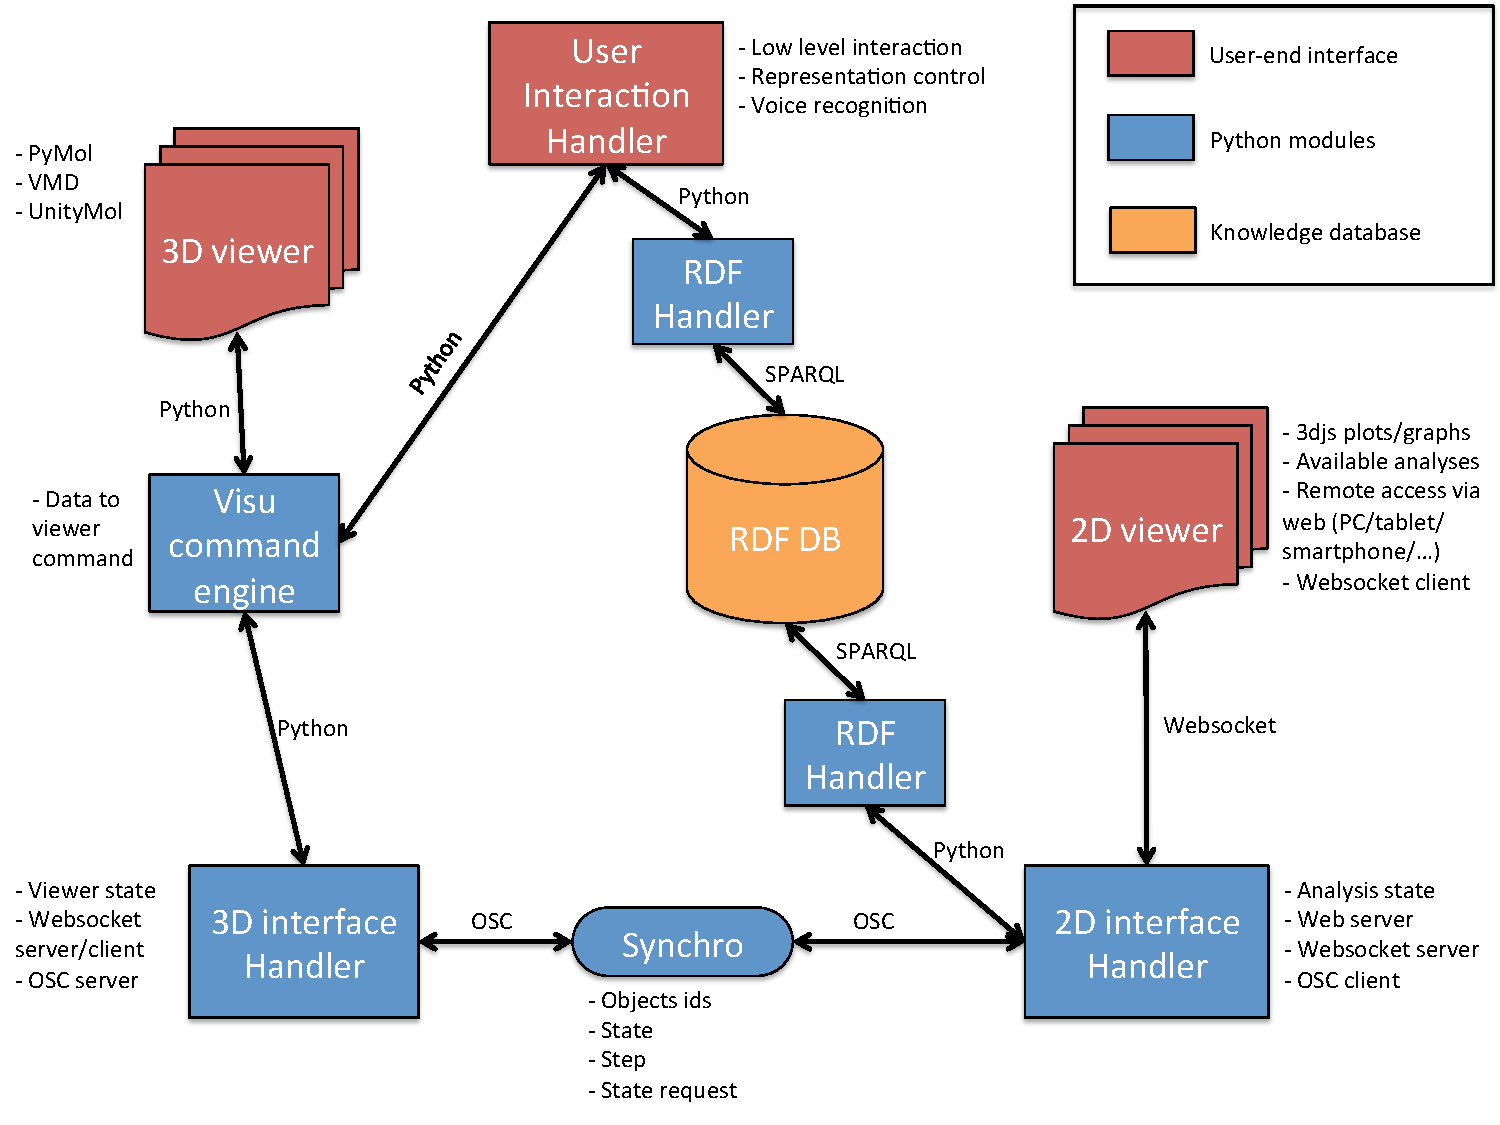
\includegraphics[width=.75\linewidth]{./figures/ch4/ch4_visu_ana_semantic_schema.pdf}}
    \caption{{\it Représentation schématique des modules et leur connectivité au sein de notre programme de visualisation analytique.}}
  \label{Fig:schema_prog_visu_ana}
  \hspace{0.3cm}
\end{figure}

\subsubsection{Composition de la commande}

Au sein de notre programme, une commande énoncée par l'utilisateur comporte comme base obligatoire une action qui décidera directement de l'événement qui sera déclenchée dans l'espace de travail. Le concept \textit{Action} comporte dans notre ontologie un certain nombre de concepts associés, sous forme de pré-requis, nécessaires à son exécution. Ces pré-requis sont indispensables car ils se comportent comme des paramètres de la commande exécutée. Une action de type \textit{Color} nécessite par exemple la présence d'une propriété de type \textit{Colors} et d'une suite de mots-clés désignant un sous-ensemble structurel. Ce sous-ensemble structurel peut être obtenu de différentes manières, dépendant directement du critère choisi par l'utilisateur pour filtrer les données sur lesquelles il souhaite appliquer son action. Une première manière de désigner un sous-ensemble structurel est la combinaison d'un composant moléculaire et d'un ensemble d'identifiant (unique, listé ou sous forme de plages continues). Sans identifiant, l'ensemble des individus appartenant au concept indiqué seront pris en compte. Une seconde manière de désigner un sous-ensemble structurel est la possibilité de combiner un composant et une propriété. Cette propriété, dont la nature n'est pas limitée, devra seulement être cohérente avec le concept édicté.
Par défaut, le sous-ensemble structurel désigné dans la commande vocale dépendra directement du jeu de données affiché dans l'espace de travail afin d'éviter une surcharge de précision à donner par l'utilisateur. Par exemple, si deux modèles sont affichés dans l'espace de travail, la commande \textit{Alanine 147} désignera uniquement les alanines dont l'identifiant est 147 parmi les deux modèles affichés et non pas parmi l'ensemble des modèles présents dans la base de données.
Si tous les pré-requis associés à une action sont présents, alors la commande est ordonnée de façon à respecter la syntaxe de l'environnement de visualisation utilisé. La dernière étape est donc une simple transformation des concepts et des individus en une formulation compréhensible par les espaces de travail.


\section{Preuve de concept}

Les différents outils présentés ici nous ont permis de mettre en place un espace de travail combinant visualisation et analyses qui repose exclusivement sur une interrogation constante de la base de données crées à partir de nos données de simulation et respectant l'ontologie OWL mise en place pour ce projet.
La conception de notre programme repose sur un schéma complexe permettant de relier efficacement ses différents composants de manière à les faire communiquer de façon optimale. La base de notre programme se trouve dans les données manipulées, toutes rassemblées au sein de la base de données RDF. Dans le schéma illustré dans la Figure \ref{Fig:schema_prog_visu_ana}, nous l'avons volontairement placé au centre d'une boucle bi-latérale de communication reliant l'espace de visualisation à l'espace d'analyse.

\subsection{Création de la base de donnée RDF}

Comme nous l'avons évoqué précédemment, nous avons mis en place une ontologie OWL regroupant l'ensemble des concepts que les experts seraient amenés à manipuler ou visualiser durant leur travail au sein de notre programme. Cette ontologie a été créée grâce à Protégé \footnote{\url{http://protege.stanford.edu/}}, une structure logicielle et éditeur d'ontologies regroupant plusieurs outils pour la création, l'édition et l'interrogation d'ontologies OWL.
Concernant la partie expérimentale, nous sommes partis de données réelles de simulation moléculaires générées par des experts du domaine. La trajectoire étudiée correspond à une dynamique moléculaire d'une protéine transmembranaire, GLIC, et d'un ligand connu pour être un de ses inhibiteurs, le bromoforme. Cette simulation de 2 nanosecondes a été effectué en solvant explicite grâce à un modèle d'eau standard, XXX et met en évidence la présence du bromoforme dans plusieurs sites de liaisons de la protéine. GLIC est une protéine responsable de la perméation de la cellule puisqu'elle régule le passage des molécules d'eau et des ions entre la partie extra- et intra-cellulaire des cellules. Plusieurs anesthésiques ont été identifié comme possédant une affinité suffisante avec GLIC pour qu'une liaison s'effectue, le bromoforme étant un des ligands concernés. La structure générale de GLIC ainsi que du bromoforme peut être observée dans la Figure \ref{Fig:glic+bromoform}. Le choix de GLIC ne fut pas anodin, trois grandes raisons ont dictées notre décision:
\begin{enumerate}
	\item C'est une protéine bien connue des experts avec lesquels nous travaillons, il est ainsi aisé d'identifié les analyses pertinentes que nous pourrons associées par la suite.
	\item La taille de GLIC est relativement importante, en particulier lorsque la membrane est représentée, nous considérons donc ce complexe comme un cas d'étude intéressant pour mettre en avant les limites de nos méthodes.
	\item L'environnement de GLIC est très hétérogène, permettant de manipuler des concepts comme les membranes et les ligands et donc de vérifier la robustesse de notre programme pour des concepts particuliers.
\end{enumerate}


\begin{figure}
  \centering
  {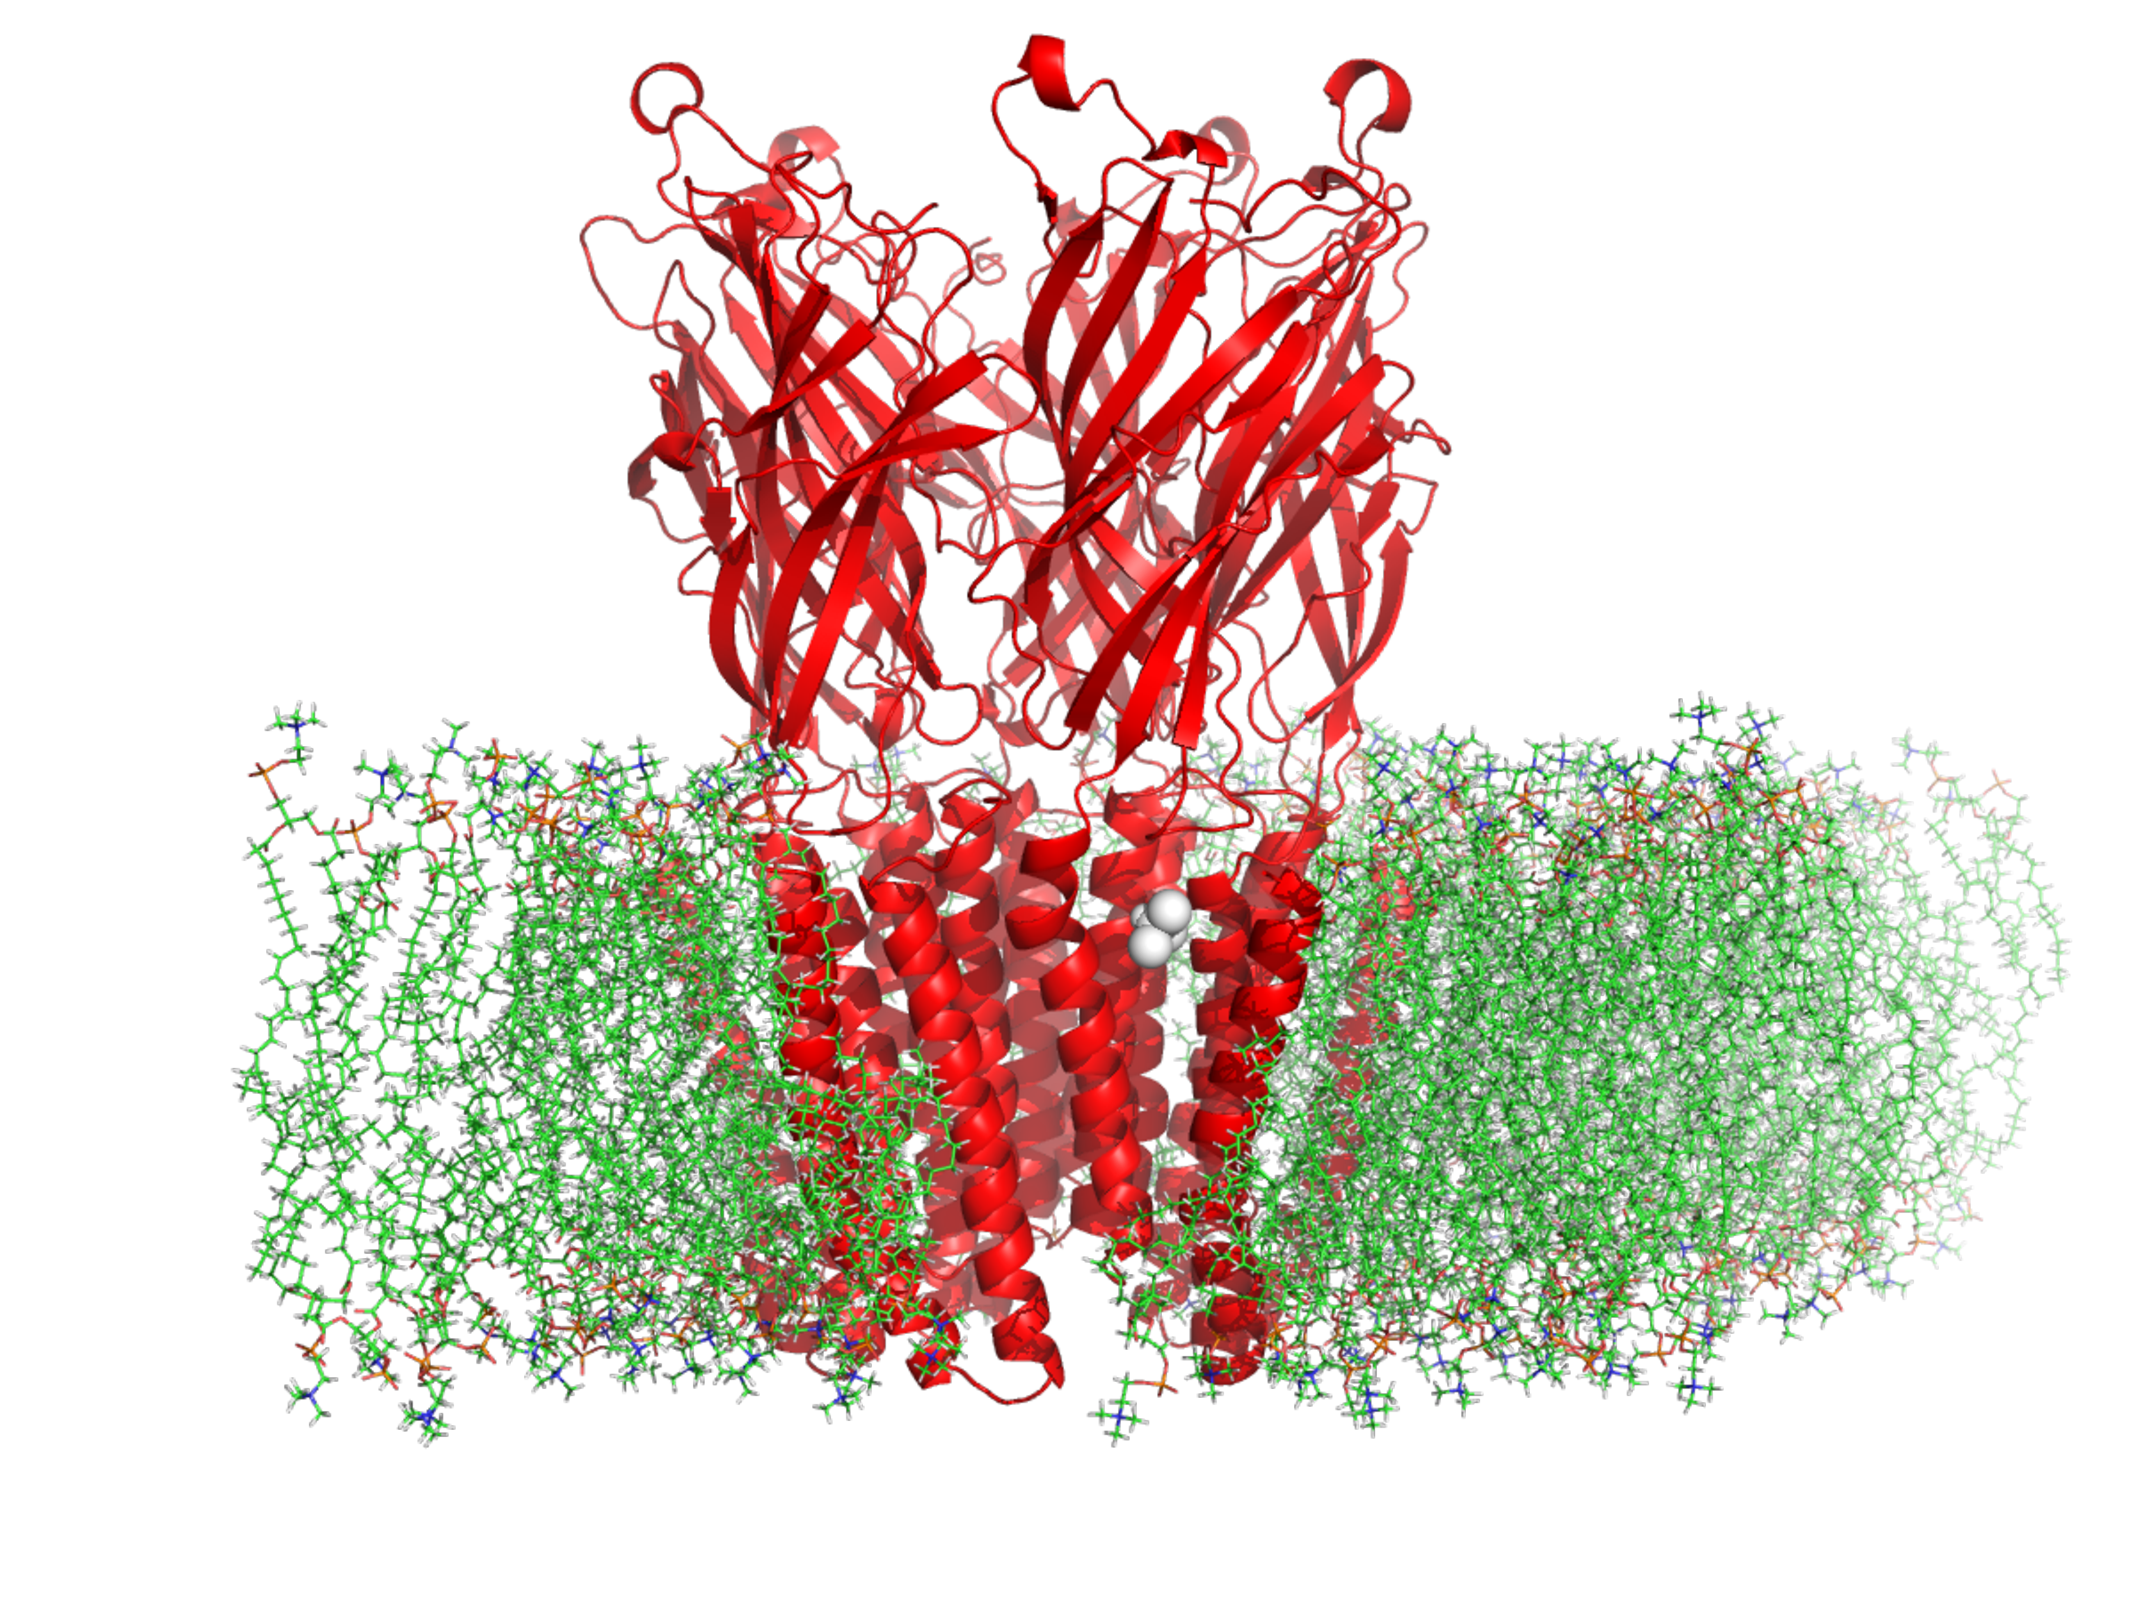
\includegraphics[width=.75\linewidth]{./figures/ch4/ch4_glic+bromoform.pdf}}
    \caption{{\it Rendu graphique de la liaison d'un bromoforme (sphères blanches) sur la protéine GLIC ("cartoon" rouge) au sein d'une membrane cellulaire (lignes vert).}}
  \label{Fig:glic+bromoform}
  \hspace{0.3cm}
\end{figure}

La transformation des données expérimentales en triplets RDF s'est faite grâce à Jena, une librairie Java permettant la manipulation de données RDF/OWL via le langage Java. Cette librairie permet de charger une ontologie sous différents formats, dont plusieurs supportés par Protégé lors de l'export, et de s'appuyer dessus afin de créer les individus correspondants aux concepts ontologiques définis. Chaque individu découle d'un ensemble de données obtenu à partir des fichiers caractérisant la simulation moléculaire étudiée. Dans notre cas, nous nous appuyons essentiellement sur des fichiers PDB décrivant la structure 3d des modèles à chaque pas de temps de la simulation. Ces fichiers possèdent les identifiants des différents groupes structurels qui seront manipulés (atomes/acides-aminés/chaînes), les coordonnées 3d des atomes ainsi que les liens des groupes structurels entre-eux. Des fichiers regroupant des données expérimentales telles que les énergies ou les températures ou bien des données analytiques comme les distances inter-atomes sont également utilisés en entrée de notre programme Java afin que leurs valeurs soient associés aux individus qu'ils décrivent. L'ontologie est faite de telle sorte qu'il soit possible d'ajouter a posteriori des valeurs physico-chimiques ou d'analyses que l'utilisateur voudrait associer à la trajectoire étudiée. Il est par exemple possible d'effectuer une analyse d'accessibilité des atomes ou des acides-aminés à la suite de la simulation et de charger les résultats pour les individus déjà existants dans la base de données. Cette possibilité nous permettra également de mettre en place des modules "optionnels" d'analyses que l'utilisateur pourra utiliser pendant sa session de travail et qui viendront ajouter les résultats obtenus directement dans la base de données pour une visualisation de ceux-ci de façon complètement intégrée. En plus du gain de temps et d'uniformisation, cela permet de sauvegarder toutes nouvelles données générées lors de la session de travail et donc de les réutiliser par la suite sans besoin de relancer les modules d'analyses ayant servi à leur création.
Les triplets créés dans Jena sont sauvegargées dans des fichiers texte sous différents formats: RDF/XML, N3 ou N-Triplets. 

Les fichiers générés, celui de l'ontologie et celui des triplets RDF, sont ensuite chargés au sein d'un serveur Virtuoso \footnote{\url{http://virtuoso.openlinksw.com/}} qui est un serveur de gestion de données dont l'architecture permet le stockage de données RDF de façon optimisée et met en place un point d'accès à ces données via un espace de requêtes SPARQL. Ce point d'accès se fait via une adresse URL que la plupart des librairies prenant en charge le SPARQL utilisent comme interface sur les données RDF. La version du serveur Virtuoso que nous utilisons permet la mise en place des règles d'inférence propres à OWL pour chaque requête SPARQL effectuée, aspect très important pour notre programme.

\subsection{Gestion des données RDF et requêtes SPARQL}

Afin de faire l'interface entre les différents modules et la base de données RDF, nous avons mis en place un module spécifique contenant un ensemble de fonctions permettant de lancer des requêtes SPARQL sur la base de données. Le nombre de fonctions est important du fait de la nature variée des informations pouvant être demandées par les modules. Cette interface sous forme de module Python utilise la librairie SPARQLWrapper \footnote{\url{https://rdflib.github.io/sparqlwrapper/}} qui permet d'accéder à tout point d'accès SPARQL via une URL, de lancer une requête et de récupérer les résultats sous format JSON, ensuite facilement convertissables en dictionnaires Python. Les résultats sont ensuite transmis aux modules ayant appelé une fonction de cette interface. Dans notre cas, le serveur Virtuoso hébergeant la base de données fournie le point d'accès SPARQL nécessaire et permet ainsi l'interfaçage du module avec la base de donnée RDF que nous avons créé.

\subsection{Visualisation des données moléculaire 3d}

Nous avons choisi PyMol \cite{delano_pymol_2002} comme programme de visualisation moléculaire 3d. PyMol est un logiciel de visualisation très utilisé dans la communauté scientifique et qui possède une API complète qui facilite son intégration au sein d'un programme modulaire complet. Nous avons utilisé cet API pour automatiser plusieurs étapes du chargement des trajectoires de simulation. Au-delà du simple chargement visuel des structures 3d de molécules et de leur rendu, nous avons mis en place au sein de PyMol des threads spécifiques surveillant les actions de l'utilisateur dans l'espace de visualisation. Plusieurs actions, dont notamment celle de sélection, peuvent déclencher un événement qui se répercutera de façon synchrone avec l'espace d'analyse. Le portage de PyMol dans des environnements immersifs est un projet en cours sous le nom "moliscope" et nous profitons des derniers développements de ce projet pour notre programme.
En plus des interactions directes comme support des actions utilisateurs, nous avons ajouté notre moteur de conversion de commandes vocales vers des commandes logicielles. Ce moteur est donc relié à PyMol afin de donner la possibilité à l'utilisateur d'effectuer plusieurs actions pré-définies de façon simple et adaptée aux environnements immersifs.
PyMol est la partie frontale de notre application, elle est reliée indirectement à un module de gestion générique qui s'occupe de recevoir et d'émettre les informations et les événements entre l'espace de visualisation et l'espace d'analyse. Ce module est construit de façon à pouvoir être relié à n'importe quel logiciel de visualisation. Il est donc indépendant de PyMol et transmet les événements liés à la visualisation à un moteur spécifique qui va s'occuper de transmettre des commandes logicielles en commandes PyMol dont la syntaxe est bien définie. PyMol pourrait donc être remplacé par un autre logiciel de visualisation moyennant une simple modification du moteur de commandes afin de l'adapter aux commandes spécifiques du logiciel utilisé.

\subsection{Visualisation des résultats d'analyses 2d}

Afin de visualiser les différents graphiques résultant des analyses effectuées a priori ou a posteriori de la session de travail, nous avons mis en place une interface web de visualisation/interaction avec ces graphiques. Nous souhaitions garantir une utilisation la plus générique possible et avec un maximum de périphériques différents. Pour ce faire, nous nous appuyons sur une librairie JavaScript de création de graphiques au sein de pages HTML appelée d3js \footnote{\url{http://d3js.org/}}. Cette librairie possède plusieurs outils de chargement de données via différentes sources, sous forme de fichiers ou à travers des flux de données. D3js permet de mettre en place des graphiques de façon relativement simple mais extrêmement paramétrables dans leur apparence ainsi que leur nature. S'appuyant sur JavaScript, elle est directement intégrée dans le code HTML d'une page web et accessible à travers toutes les plateformes permettant de visualiser du contenu HTML.
Nous utilisons un serveur web basé sur une librairie python, Flask, afin de mettre en place notre environnement web. Flask permet la création d'un server web via la création d'un accès web local. L'environnement HTML et JavaScript est automatiquement pris en compte par la librairie qui s'appuie sur les fichiers utilisateurs ordonnés au sein d'une hiérarchie de dossiers propres à la librairie. Plusieurs extensions existent dont Flask-SocketIO qui permet aux applications Flask d'accéder à une communication bi-directionnelle et de faible latence entre le serveur et le client web. Côté client, il suffit d'utiliser la librairie JavaScript SocketIO pour pouvoir envoyer et recevoir des messages vers ou depuis le serveur web Flask. Une connexion permanente peut ainsi être mise en place entre le client et le serveur.
La plupart des événements d'interaction déclenchés par l'utilisateur au sein de la page HTML et des graphiques d3js peuvent ainsi être répercutés directement au serveur web. Suivant la nature des événements, le serveur renvoie ensuite les informations aux modules concernés.
L'espace de visualisation des résultats d'analyses est divisé en niveaux hiérarchiques structuraux qui correspondent à ceux référencés dans l'ontologie: \textit{Model} / \textit{Chain} / \textit{Residue} / \textit{Atom}. Les graphiques dessinés dans chaque niveau correspondent à des individus du niveau hiérarchique représenté. Afin de garder une cohérence entre les graphiques représentés, chaque sélection effectuée dans un graphique entraîne une mise à jour des graphiques présents dans les niveaux hiérarchiques inférieurs. Cette mise à jour se fait grâce à une requête émanant du script JS relayée ensuite au module de gestion RDF qui lancera une requête SPARQL pour les propriétés affichées dans les graphes mis à jour mais seulement pour les individus sélectionnés par l'utilisateur.

\subsection{Analyses semi-automatiques}

Bien que la majorité des données soient présentes au sein de la base de données créée par l'utilisateur, une session de travail habituelle génère souvent des données résultantes de calculs post-simulation et donc absentes de la base de données de départ. Ces calculs sont habituellement gérés au sein de scripts, liés ou non aux outils de simulation, et exécutés en dehors de la boucle de visualisation suite à l'observation de phénomènes particuliers lors de l'exploration des structures de la simulation ou suite à d'autres analyses déjà effectuées auparavant. Afin de ne pas surcharger la base de données et laisser l'utilisateur maître des analyses qu'il veut effectuer, nous avons profité de notre connaissance métier pour mettre en place la possibilité de lancer certaines analyses semi-automatisées pendant la session de travail. Ces analyses semi-automatisées se basent essentiellement sur les analyses utilisées usuellement par les experts du métier. Au-delà de la simple proposition d'une liste d'analyses pouvant être lancées à la volée, la connaissance du système étudié grâce à sa base de données RDF associée nous permet de proposer, pour plusieurs analyses, des données d'entrée filtrées et identifiées sur lesquelles appliquer les analyses désirées. L'outil \textit{distance} nécessite par exemple deux individus de même niveau hiérarchique structural ainsi qu'une sélection d'individus de niveau hiérarchique supérieur au sein desquels seront calculés ces distances. Il est possible de classer ces analyses en deux catégories: Les analyses simples regroupent les analyses où chaque individu possède une unique valeur de la propriété calculée. Parmi celles-ci nous pouvons citer l'accessibilité au solvant, l'hydrophobicité, l'énergie, etc. 
Les analyses complexes sont elles le résultat d'une propriété nécessitant la présence de plusieurs individus pour être pertinentes. Nous pouvons citer parmi les analyses complexes entre deux individus la distance, le RMSD, l'angle, etc.

Alors que les analyses simples ajoutent simplement à un individu une propriété et la valeur associée, les analyses complexes doivent elles créer un individu particulier d'un des concepts \textit{Analyse} de l'ontologie qui regroupera les informations nécessaires à sa compréhension. Le concept \textit{Distance} (de type \textit{Analyse}) de l'ontologie permettra par exemple de stocker toute distance calculée entre deux individus pour une sélection de structures parentes définies. La valeur de la distance, l'URI des deux individus impliqués ainsi que l'ensemble des structures au sein desquelles le calcul s'est effectué seront des propriétés d'un individu \textit{Distance} et seront accessibles seulement à travers cet individu. Cela ne complexifie donc pas seulement le stockage mais également l'accès aux informations puisque les valeurs d'analyses complexes ne sont, au contraire des analyses simples, plus directement associées aux individus concernés mais à travers un concept \textit{Analyse} intermédiaire. Il fut donc nécessaire d'adapter les requêtes SPARQL utilisées pour la génération des graphes afin de prendre en compte cette complexité. La différence entre une requête SPARQL accédant aux valeurs d'une analyse simple et la requête SPARQL permettant d'accéder à celles d'une analyse complexe est illustrée dans le Listing \ref{sparql_simple_vs_complexe}.

\begin{lstlisting}[language=XML, caption=Deux requêtes SPARQL: 1. Accès à la température d'un modèle 2. Accès à la distance entre deux résidus, label=sparql_simple_vs_complexe]
SELECT DISTINCT ?temp WHERE {my:MODEL_161 my:temperature ?temp}

SELECT DISTINCT ?distance WHERE {?indiv rdf:type my:Distance . ?indiv my:objectA my:RES_3622 . ?indiv my:objectB my:RES_3626 . ?indiv my:distance ?distance}
\end{lstlisting}

\subsection{Synchronisation}

La nature hétérogène des modules de notre application nous empêche d'adopter une communication directe entre les différentes instances Python créées par les différents modules. Flask et PyMol ont tous les deux besoin de fonctionner dans un processus principal au sein desquels d'éventuels sous-processus peuvent se greffer. Ils ne peuvent donc pas être utilisés au sein de la même boucle de calcul et nécessitent d'être initialisés de façon indépendante. La synchronisation entre l'espace visuel et l'espace d'analyses, représenté respectivement par PyMol et le serveur web Flask, se fait au travers de communication entre leurs modules de gestion respectifs. Cette communication s'appuie sur des messages OSC envoyées par les modules à chaque événement déclenché dans un des espaces de travail. Chacun des modules est ainsi associé à un serveur OSC opérant en arrière-plan dans un sous-processus et surveillant tout message arrivant sur le port qui lui est dédié. Nous utilisons la librairie Python pyliblo \footnote{\url{http://das.nasophon.de/pyliblo/}} qui est une interface Python pour liblo \footnote{\url{http://liblo.sourceforge.net/}}, une implémentation du protocole \textit{Open Sound Control} (OSC). OSC est un format de transmission de données conçu pour être utilisé en temps réel. Il utilise des protocoles UDP ou TCP à travers le réseau et permet d'envoyer des messages de différents typages suivant les besoins. Pyliblo, en plus de permettre la création d'un serveur OSC, fournit également les fonctions nécessaires pour envoyer un message. Ces messages sont envoyés localement sur un port ouvert référencé par la machine qu'un serveur OSC "surveille" afin de détecter tout message entrant. La destination des messages n'est pas renseignée uniquement par le port UDP d'arrivée, il est également possible de fournir un chemin particulier. Cette adresse définie au préalable agit comme un premier filtre de distinction entre les messages de différentes natures. Le typage des messages suivant les adresses est strict et prédéfini dans le module du serveur OSC. Un message contenant une chaîne de caractères à une adresse précise ne sera donc pas traitée dans la même méthode qu'un message adressé à la même adresse mais dont le contenu est un tableau d'entiers.
Les communications constantes entre les modules à travers les ports UDP de nos serveurs OSC permettent donc d'assurer une synchronisation des actions utilisateurs dans chacun des espaces de travail. Les actions identifiées comme synchronisables sont donc effectuées en coordination entre les espaces.
A chaque création de graphique dans l'espace de visualisation, l'information de création est envoyée afin de créer un objet \textit{Selection} qui regroupera les information de sélection effectuées au sein du graphique correspondant. Cet objet est référencé au sein de la base de données RDF et contient: Le niveau hiérarchique structural des individus, les individus sélectionnés dans le graphique, la représentation géométrique associée et le rendu visuel appliqué (couleur et transparence). Ce stockage permet de sauvegarder l'état de la visualisation à tout moment et de la corréler aux analyses présentées au sein de l'espace d'analyse. De plus, un découpage des graphiques en objet \textit{Selection} permet à l'utilisateur de choisir quels groupes de sélection il désire afficher ou cacher au sein de l'espace de visualisation par simple cochage d'une case associée à chaque graphique. Il est donc possible de superposer les rendus visuels de chaque graphique ou d'une partie seulement suivant la volonté de l'utilisateur. Ces objets \textit{Selection} sont mis à jour à chaque interaction de l'utilisateur dans le graphique correspondant afin de refléter les individus sélectionnés. La possibilité de sauvegarder l'état de visualisation et des analyses présentes ainsi que des individus sélectionnées permet naturellement de charger un état précis d'une session de travail. Ceci est d'une grande importance lorsque l'état des espaces de travail a été atteint après une succession longue et précise d'étapes.

Parmi les différentes techniques de visualisation analytique citées dans la section \ref{visu_ana_tools}, celle du Focus+Context, et plus spécifiquement de la technique du \textit{brush-and-link}, est un candidat pertinent pour mettre en avant des informations supplémentaires obtenues à partir des analyses indépendantes effectuées sur une simulation. En biologie structurale, les résultats d'analyse peuvent souvent être représentés au travers de nuages de points, d'histogrammes ou de diagrammes à bandes. Ces représentations s'adaptent particulièrement bien à la technique du \textit{brush-and-link} puisque la sélection de sous-ensembles y est aisée. De plus, la perspective d'une fenêtre dynamique regroupant le contexte global et les détails dans un même ensemble est particulièrement adapté à un environnement immersif. En effet, l'immersion peut être considérablement impactée, et ce de façon négative, lors du partage spatial du dispositif immersif en plusieurs contextes de travail.
Du point de vue de la visualisation, le but est d'être capable de sélectionner un sous-ensemble structural d'un complexe moléculaire afin de mettre en avant les informations correspondant à ce sous-ensemble dans l'espace d'analyses. Par exemple, et comme illustré dans la Figure \ref{Fig:bilateral_selection}, la sélection d'un ou plusieurs modèles de la trajectoire aura pour conséquence de mettre en avant cette sélection au sein de la structure et de mettre en avant le sous-ensemble, si existant, dans les graphiques d'analyse. Chaque point des graphiques est relié à un niveau hiérarchique structural précis (modèle/chaîne/résidu/atome) et une action sur un ensemble de points aura pour effet d’entraîner une action sur le niveau structural correspondant. 


\subsection{Exemples}

\subsubsection{Scénario I}

Un exemple d'utilisation de notre application est illustré dans la figure X.

Dans le scénario choisi, le premier événement pris en compte au sein de l'application est le choix de l'utilisateur quant aux analyses qu'il désire afficher. Ce choix lancera une première paramétrisation de l'espace d'analyse qui pourra ainsi se connecter à l'espace de visualisation. 
Il est cependant possible de démarrer une session de travail par une exploration de la trajectoire étudiée mais cette exploration ne déclenchera pas d'événements dans l'espace visuel, ce dernier n'étant pas paramétré.
Le choix des analyses se déroule sur la page HTML et va interroger de façon quasi instantanée la base de données RDF par l'intermédiaire du serveur web et via des requêtes SPARQL transmises du module de gestion RDF. La première requête vise à identifier les propriétés pour lesquels une valeur littérale existe pour le groupe structurel d'intérêt choisi par l'utilisateur. Ces valeurs littérales peuvent provenir de données structurales pures générées par GROMACS lors de la simulation moléculaire ou bien d'analyses post-simulations ayant été intégrées au sein de la base de données. Toutes les propriétés possédant une valeur littérale sont donc affichées dans deux colonnes. Une colonne permet de choisir la propriété à afficher sur l'axe des abscisses, la seconde colonne désigne la propriété qui sera affiché sur l'axe des ordonnées. L'utilisateur a la possibilité de choisir plusieurs combinaisons de propriétés à afficher sous forme de graphes. Quand son choix est terminé, une requête SPARQL est envoyé à la base de données pour récupérer les valeurs des propriétés choisies. Ces données sont ensuite mises sous forme de graphes et structurées grâce à d3js.
Lorsque les graphes sont générés, l'utilisateur a la possibilité d'interagir avec eux de différentes manières: 
\begin{itemize}
	\item Il peut sélectionner un point unique dans un des graphes afin d'obtenir des informations plus précises via un cadre rassemblant les informations contenues dans la base de données pour l'individu sélectionné.
	\item Il est possible de sélectionner un ensemble de points dans un des graphes et afficher un cadre d'information rassemblant plusieurs statistiques sur l'ensemble des propriétés des individus ainsi sélectionnés (moyenne, écart-type, pourcentages, etc.).
	\item Il est également possible de synchroniser la sélection d'un groupe de points afin de mettre en évidence les individus concernés dans l'ensemble des graphes de la page.
\end{itemize}

Toute sélection au sein d'un ou plusieurs graphes de la page déclenche un événement transmis depuis le client web jusqu'au module de gestion 3d entraînant une adaptation de la visualisation pour mettre en avant le ou les individu(s) ayant été sélectionnés. Il est aussi possible d'obtenir, sous forme de fenêtre indépendante, un résumé des informations disponibles sur le ou les individus. Dans le cas d'un individu unique, une liste de ses propriétés et de leurs valeurs sera affichée alors que pour plusieurs individus, une moyenne effectuée sur les valeurs de leurs propriétés remplacera les valeurs brutes.
Chaque sélection réduit donc le focus de l'utilisateur à un sous-ensemble d'individus, à la fois dans l'espace d'analyses mais également de façon synchrone dans l'espace de visualisation. Il est possible d'adapter ce focus suivant les besoins de l'utilisateur en modifiant le niveau de contexte dans lequel il désire que sa sélection apparaisse. Trois niveaux de contextualisation sont possibles:
\begin{itemize}
	\item Aucun contexte - La sélection d'individu(s) entraîne la visualisation unique de ces individus dans l'espace de visualisation et d'analyse et donc cache tout individu n'étant pas sélectionné
	\item Contexte faible - La sélection d'individu(s) met en avant ces individus dans les espaces de travail et réduit la perception des autres individus du jeu de données (couleur grise, transparence, rendu visuel simplifié, etc.)
	\item Contexte fort - La sélection d'individu(s) n'est perçu qu'à travers une mise en avant simple de ces individus dans les espaces de travail. Tout autre individu apparaîtra également avec des paramètres visuels proches des individus sélectionnés.
\end{itemize}

Ces différents niveaux permettent soit de mettre en évidence les différences entre la sélection et le reste du jeu de données, soit de mettre en place un environnement de travail épuré sur une sélection d’intérêt pour l'utilisateur. Ces niveaux s'appliquent à la fois pour la partie visuelle et analytique via des systèmes de rendus visuels propres à chaque espace.

Lorsque une sous-sélection d'individus est effectuée, l'utilisateur a toute liberté pour l'explorer dans l'espace de visualisation. Si, lors de son exploration, l'utilisateur désire sélectionner un sous-groupe plus précis au sein des individus affichés, il possède deux manières de le faire. Soit via une sélection directe via une commande gestuelle avec ou sans appareil d'interaction associé, soit par commande vocale en verbalisant le sous-groupe d’intérêt via la commande \textit{Select}.
Au-delà du changement visuel induit par la sélection dans l'espace de visualisation, ce changement va également produire un rafraîchissement de l'affichage de l'espace d'analyses, de la même manière que la précédente sélection effectuée dans l'espace d'analyses induisait une synchronisation dans l'espace de visualisation. Ici, deux possibilités sont présentes. La première est que l’utilisateur désire conserver le niveau structurel de sélection qu'il avait adopté dans la première étape. Dans ce cas, le changement de l'espace d'analyse sera uniquement une mise à jour du sous-groupe d'individus à mettre en avant au sein des différents graphes. La seconde possibilité est que le niveau structurel de sélection diffère du niveau précédent. Dans ce cas, les graphes ne portent pas l'information de ce niveau structurel précis et doivent donc être rechargés pour de nouvelles valeurs, correspondant au niveau structurel désiré. Ce comportement est le comportement par défaut de l'espace d'analyses, cependant, il peut être modifié afin de garder les informations précédentes et donc de couper la synchronisation avec l'espace de visualisation. Dans ce mode asynchrone, aucune action effectué dans chacun des espaces n'aura d'influence sur le second espace. La synchronisation se réactivera à tout moment lorsque les niveaux structurels des deux espaces seront identiques.
Alors que le mode asynchrone est activable à tout moment, il n'est pas possible de forcer le mode synchrone puisqu'une incohérence existera entre les informations demandées dans un espace et celles présentées dans le second espace.

\section{Résumé et conclusion}
\label{sec:ConclusionVisuAna}

Afin d'optimiser le travail autour de l'étude de structures moléculaires au sein d'un environnement immersif, nous avons développé une suite logicielle basée une communication bi-latérale entre deux espaces indispensables en biologie structurale: un espace de visualisation et un espace d'analyses. Cette communication entre deux espaces aux caractéristiques différentes est rendue possible grâce à la représentation haut-niveau de l'ensemble des concepts avec lesquels l'utilisateur interagit lors d'une session de travail. Ces concepts peuvent être aussi bien scientifiques, et concernés les données manipulées et observées, que logiciels, décrivant les composants et les actions de la plateforme choisie. L'ontologie créée permet une homogénéité des données échangées entre l'ensemble des modules de calculs (rendu visuel, analyses, simulation) puisque chaque module peut accéder aux données qu'il utilise au sein de la base de données construite autour de l'ontologie. On retrouve cette notion d'homogénéité en dehors de l'utilisation même de l'application puisque la représentation ontologique des concepts permet également d'assurer une cohérence et un modèle commun de données à respecter par les utilisateurs lors de la mise en place de nouvelles bases de données de complexes moléculaires. Ainsi, il est possible de mettre en commun certaines informations et d'enrichir les connaissances grâce à des requêtes croisées SPARQL par exemple. La communication inter-modules est la clé de voûte de notre application et l'approche passant par représentation sémantique des données favorise grandement sa mise en place. Cette approche n'a pas pour seul effet de garantir la cohérence des données échangées, elle permet aussi une certaine anticipation de certaines actions de l'utilisateur et donc de mettre en place des processus d'interaction plus simples et plus directes correspondant parfaitement aux environnements immersifs dans lesquels nous travaillons.
Notre application, malgré la présence de multiples communications entre les modules, respecte les contraintes temporelles inhérentes à tout application interactive. La figure X montre les temps d'exécution des principales actions utilisateurs lors d'une session de travail. On constate qu'elles sont toutes réalisables dans un temps considéré comme interactif puisque de l'ordre de ce que l'on pourrait attendre pour une application standard.
Les bases de données sont un excellent moyen de stocker et mettre à disposition à tout instant les informations obtenues par l'utilisateur lors de ses sessions immersives de travail. Chaque nouvelle analyse met en jeu des résultats qui seront automatiquement stockés dans la base de données et réutilisables par la suite. Ceci assure une continuité dans le travail et permet de reprendre toute session à un point bien particulier. Les possibilités de partager ainsi une session de travail entre collaborateurs ou de reprendre une session de travail à l'état où elle se trouvait lors de sa dernière utilisation sont des caractéristiques que la majorité des scientifiques apprécient lors de l'utilisation de leurs outils. L'étude de l'évolution de structures moléculaires est un processus long et, comme évoqué précédemment, structuré en boucles successives, il est donc important d'être capable d'avoir un suivi stricte du travail effectué. La communication est également un enjeu majeur dans les sciences où le partage des informations entre collaborateurs et scientifiques du même milieu est primordial puisqu'elle constitue une partie des processus d'évaluation. Il est possible d'aller plus loin dans ce partage d'informations au sein de notre application en développant l'aspect collaboratif. La mise en place d'un formatage stricte des états de visualisation dans un format lisible et utilisable par notre application pourrait permettre la sauvegarde de toute évolution sous forme de fichiers, partageables ensuite dans d'autres environnements. L'une des forces de notre application repose également sur son développement autour d'une base de données construite autour d'une ontologie précise. Les modules au coeur de l'application n'ont aucune connaissance des logiciels ou librairies utilisés pour l'affichage 2d et 3d. Cette dissociation permet le couplage d'un nombre important de logiciels de visualisation 3d et 2d. Ce couplage passerait par un simple portage des modules de conversion des données en commandes spécifiques pour les logiciels de visualisation choisis.


